\documentclass[11pt,a4paper]{article}
\usepackage[T1]{fontenc}
\usepackage{lmodern}
\usepackage[margin=2.4cm]{geometry}
\usepackage{microtype}
\usepackage{amsmath}
\usepackage{graphicx}
\usepackage{booktabs}
\usepackage{tabularx}
\usepackage{xcolor}
\usepackage{tikz}
\usepackage{pgfplots}
\pgfplotsset{compat=1.18}
\usepackage{textcomp}
\usepackage[font=small,labelfont=bf]{caption}
\usepackage{enumitem}
\setlist{itemsep=1pt,topsep=3pt}
\usepackage{xurl}
\usepackage[colorlinks=true,linkcolor=blue!50!black,urlcolor=blue!50!black,citecolor=blue!50!black]{hyperref}
\newcommand{\degC}{\,\textdegree{}C}
\renewcommand{\arraystretch}{1.15}

\title{\textbf{CropShift Earth}\\[4pt]
\large Separating real climate trends from year-to-year noise,\\ and what they mean for crops in the Middle East and North Africa}
\author{Team Tech Ghosts\\[2pt]
\normalsize NASA Space Apps Challenge 2026, Cairo\\
\normalsize Challenge: \emph{Be An Earth System Trend Detective!}}
\date{15 November 2026}

\begin{document}
\maketitle

\begin{abstract}
\noindent A few unusually hot summers do not make a trend, yet most climate dashboards leave it to the reader to tell the two apart. We built CropShift Earth, a web globe that takes 25 years of monthly NASA POWER data (2001 to 2025) and, for any place, country or the whole Earth, reports how fast a variable is changing, where, since when, and how strong the statistical evidence is. Significance is tested with a Mann--Kendall test whose variance is corrected for year-to-year persistence, and every map is controlled for false discoveries. We chose this method by simulation: of seven candidates it kept false alarms close to the nominal 5\% while losing much less detection power than pre-whitening. The trend engine reproduces NASA GISTEMP's global warming rate ($+0.25$\degC{} per decade, $p<0.001$) and agrees in direction with NASA's station record over 87\% of the Earth's area. For 20 countries of the Middle East and North Africa we then ask a practical question: which of 40 crops fit a place today, and in 2030 and 2035 if current trends continue? A gradient-boosted model trained on where crops are grown worldwide answers it with a held-out AUC of 0.90.
\end{abstract}

\begin{center}\small
\begin{tabularx}{0.94\linewidth}{@{}lX@{}}
\toprule
\textbf{Live app} & \url{https://cropshift-earth.onrender.com} \\
\textbf{Project page} & \url{https://www.spaceappschallenge.org/2026/find-a-team/tech-ghosts/} \\
\textbf{Demo video} & linked on the project page (30 seconds) \\
\textbf{Source code} & \url{https://github.com/spaceapps-cairo-2026/nasa-space-apps-2026} \\
\textbf{Crop model} & \url{https://huggingface.co/OmarGhost2005/cropshift-earth-crop-model} \\
\textbf{API documentation} & \url{https://cropshift-earth.onrender.com/docs} \\
\bottomrule
\end{tabularx}
\end{center}

\section{Introduction}

Ask a farmer near Asyut whether summers are getting hotter and the answer will usually be yes. Ask whether the change is real or just a run of bad years, and the honest answer is that nobody has checked. Climate records are noisy: a single El Ni\~no year, a heat wave or a dry winter can move a 25-year average more than a decade of slow warming does. Drawing a straight line through the data is easy. Deciding whether that line means anything is the hard part, and it is the part most public tools skip.

The question matters more in some places than in others. The Middle East and North Africa is the most water-scarce region in the world \cite{worldbank2018}, the Mediterranean basin is already about 1.5\degC{} warmer than in pre-industrial times \cite{medecc2020}, and in Egypt 17.5\% of all workers are employed in agriculture \cite{owid}. For a farmer, an investor or a ministry, ``the climate is changing'' is not enough. They need to know where the change is established, how large it is, and what it implies for the crops they grow.

The challenge \emph{Be An Earth System Trend Detective!} asks for a tool that lets users choose variables from NASA missions or models, see how they change over time, and determine what is changing, where, by how much, and whether the change is significant. It also points out that one physical process can push the same variable in opposite directions in different regions. CropShift Earth answers each of these questions for any place on Earth, and adds one step that we think is missing from most trend tools: translating established trends into crop suitability for the region we live in. Our main contributions are:
\begin{itemize}
\item a trend engine whose false-alarm rate we measured before choosing it, applied with false discovery control to every map;
\item an independent check of our results against NASA's station and satellite records, including a data problem we found and handled;
\item a crop suitability outlook for 40 crops in 20 countries, today and under continued trends to 2035.
\end{itemize}

\section{Data}

\paragraph{NASA POWER.} All maps, charts and crop scores are computed from NASA POWER monthly data \cite{power}, which is derived from NASA's MERRA-2 reanalysis \cite{gelaro2017} on a $0.5^\circ \times 0.625^\circ$ grid (about 55\,km). We use six variables for 2001 to 2025: air temperature at 2\,m (\texttt{T2M}), its daily maximum (\texttt{T2M\_MAX}), precipitation (\texttt{PRECTOTCORR}), relative humidity (\texttt{RH2M}) and surface and root-zone soil wetness (\texttt{GWETTOP}, \texttt{GWETROOT}); daily minimum temperature (\texttt{T2M\_MIN}) is used for single points. Monthly values are averaged into yearly means before any test. Data for a new region are fetched from NASA on first use and cached; Egypt and a global air temperature grid ship with the application.

\paragraph{Independent records.} To check our results we use NASA GISTEMP v4 \cite{lenssen2019}, both the global mean and the 250\,km gridded station anomalies, and the GPCP v2.3 monthly precipitation analysis, which combines satellites and rain gauges \cite{adler2018}.

\paragraph{Crops.} Where crops are grown today comes from IFPRI's MapSPAM 2020 v2r2 \cite{spam2020}, aggregated onto the POWER grid (22,450 farmland cells on every continent). FAOSTAT's list of crops grown in Egypt \cite{faostat} is used only as an independent check. Country borders and city names come from Natural Earth, and the globe uses NASA GIBS imagery.

\section{Methods}

\subsection{Rate of change}
For each grid cell or point we estimate the rate of change with the Theil--Sen slope \cite{sen1968}, the median of all pairwise slopes between years. It is robust to the one-off extreme years that are common in this kind of data. We report it per decade, in the variable's own units, with a 95\% confidence range.

\subsection{Is the change real?}
We test for a monotonic trend with the Mann--Kendall test \cite{mann1945,kendall1975}. Yearly climate series are often persistent (a warm year tends to follow a warm year), which makes the plain test report trends that are not there. We therefore scale the test's variance by an effective sample size derived from the lag-1 autocorrelation \cite{hamed1998,yue2004}. For series of 20 years or more the autocorrelation is measured on the residuals from a quadratic fit, so that a change that bends (flat, then rising) is not mistaken for persistence.

A map tests hundreds of cells at once, and at the 5\% level about one cell in twenty would look significant by chance alone. We control this with the Benjamini--Hochberg false discovery rate \cite{bh1995}, as recommended for climate maps by Wilks \cite{wilks2016}. The app reports three levels: \emph{strong evidence} ($q<0.01$), \emph{moderate evidence} ($q<0.05$) and \emph{not proven}. The number itself is always shown, phrased as ``Could this be luck?'': how often a trend this strong would appear if nothing were changing. ``Not proven'' is never presented as ``no change''. Finally, the Pettitt test \cite{pettitt1979} estimates the year a shift started when there is one ($p<0.05$).

\subsection{How we chose the method}
We did not want to pick a test because it is popular. We generated 20,000 synthetic 25-year series, with and without a trend and with different degrees of persistence $\rho$, and ran seven candidate methods on them. Table~\ref{tab:methods} shows part of the outcome. The plain test and the widely used Hamed--Rao correction raise false alarms in about a quarter of trendless series once persistence is strong. Pre-whitening keeps false alarms low but finds fewer than a third of real trends. The effective-sample-size correction we use stays between 3.3\% and 8.8\% and still finds two thirds of the stronger trends, the best balance among the methods we compared on both measures. The price is caution: with only 25 years, a real but small trend is often reported as not proven.

\begin{table}[h]\centering\small
\caption{Candidate trend tests on 20,000 synthetic 25-year series. False alarms: share of trendless series called significant at $p<0.05$ (fair value 5\%). Detection: share of series with a real trend (total change 2.5 times the yearly noise, $\rho=0.3$) that are found.}\label{tab:methods}
\begin{tabular}{@{}lccc@{}}
\toprule
Method & False alarms, $\rho=0$ & False alarms, $\rho=0.6$ & Detection \\
\midrule
Plain Mann--Kendall & 4.5\% & 28.2\% & 88.5\% \\
Hamed--Rao, all lags & 7.9\% & 25.2\% & 86.2\% \\
Pre-whitening & 3.8\% & 5.3\% & 29.6\% \\
Trend-free pre-whitening & 4.5\% & 34.3\% & -- \\
Effective sample size (chosen) & 3.3\% & 8.8\% & 67.0\% \\
\bottomrule
\end{tabular}
\end{table}

\subsection{Crop suitability model}
For each of 40 crops we trained an XGBoost classifier \cite{chen2016} to tell grid cells where the crop is grown (at least 2\% of the harvested area, or 500\,ha) from cells where it is absent. Each cell is described by ten climate features computed from all six POWER variables (for example mean and coldest-month temperature, hottest monthly maximum, annual rainfall and its seasonality, humidity and soil wetness) plus the share of irrigated land. Irrigation is an input, so the same model answers both ``irrigated'' and ``rain only''. Deserts with almost no rain were added as counter-examples, and in rain-only mode scores fade to zero below 100\,mm of rain a year, because no crop is grown on rain alone there. Models were selected by spatial block cross-validation on $10^\circ \times 10^\circ$ blocks, so that the score always comes from regions the model did not see. The 8,000 trees are packed into a small file that runs with NumPy alone.

\subsection{Projections}
Each of the ten climate features is extended along its own 2001--2025 Theil--Sen trend to 2030 and 2035, and the crop model is applied to the projected climate. A 95\% range comes from 200 block-bootstrap resamples of the years. These are explicitly scenarios of the form ``if current trends continue'', not forecasts. For rain, humidity and soil wetness we first remove a one-time step in the POWER record around 2015 (Section~\ref{sec:rain}).

\section{Implementation}
The analysis is written in Python and served by a FastAPI application whose endpoints are documented online. The interface is a browser application (MapLibre GL JS globe, Plotly charts, plain JavaScript) with four tabs: Trends, Crops, Farmland and Decisions, plus a page explaining the methods and a 60-second guided tour (Figure~\ref{fig:app}). Sixty-nine automated tests run on every change. The application is hosted on Render and the crop model is published on Hugging Face.

\begin{figure}[h]\centering
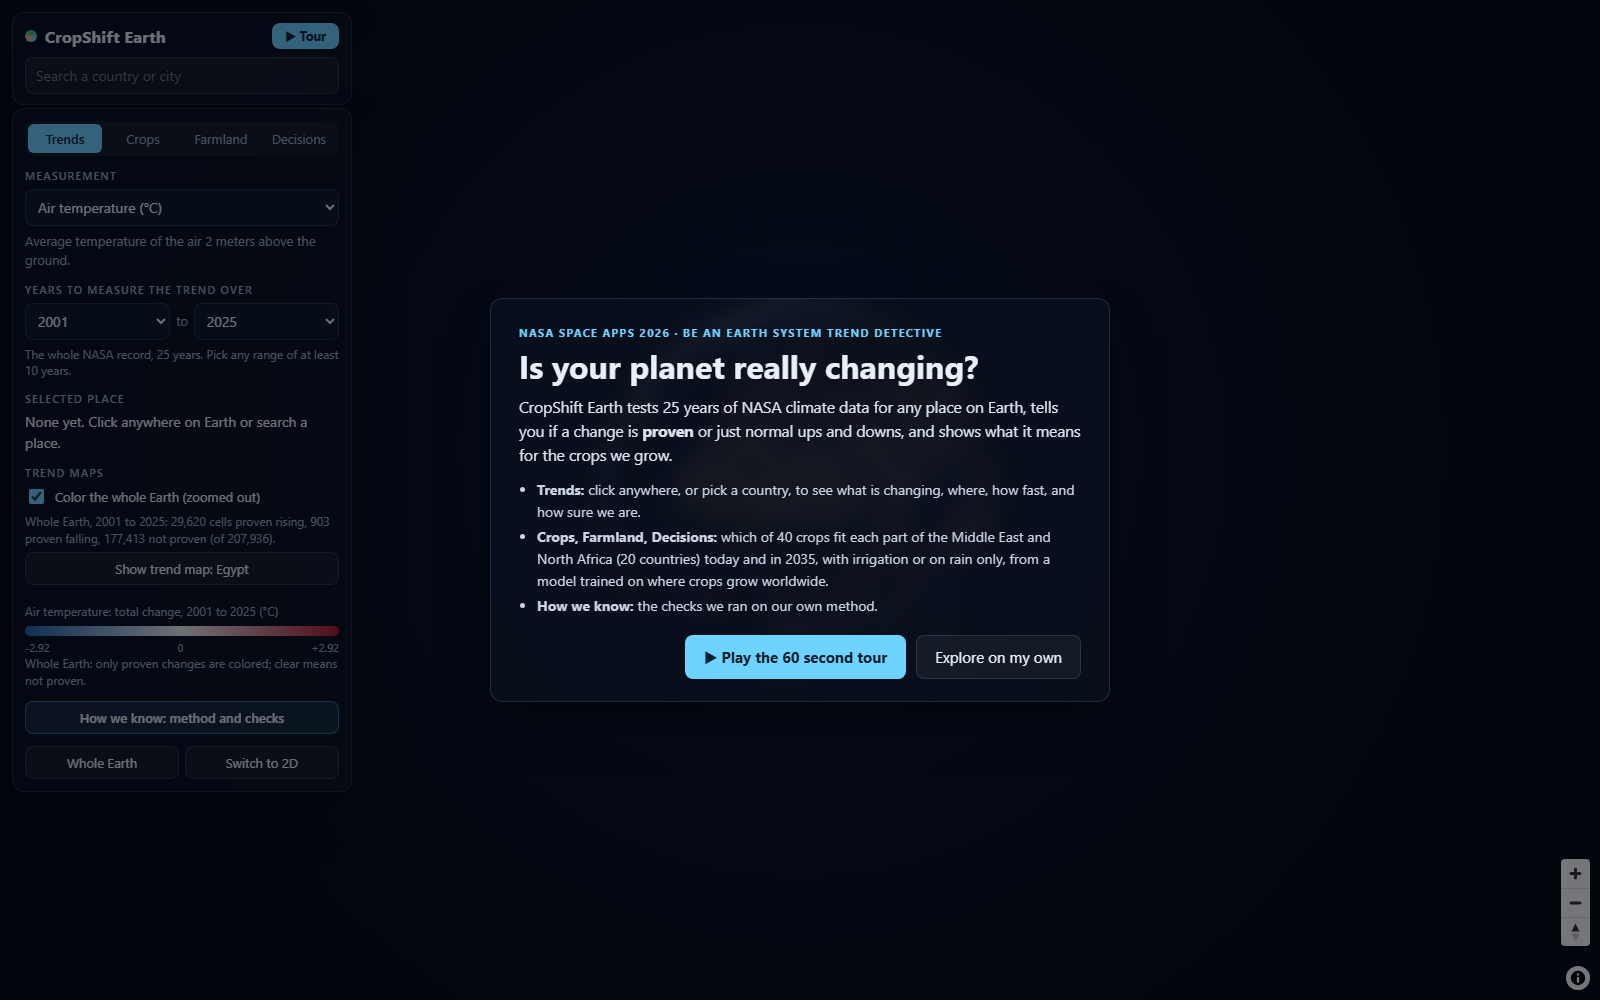
\includegraphics[width=0.9\linewidth]{app_welcome.png}
\caption{Start screen of the live application. The left panel already reports the global result for air temperature, 2001 to 2025: 29,620 cells with proven warming, 903 with proven cooling and 177,413 not proven, out of 207,936.}\label{fig:app}
\end{figure}

\noindent All of the following works in the deployed version: point and city trends anywhere on Earth with the matching station trend for air temperature; trend maps for any country or region; the whole-Earth layer; any period of at least ten years between 2001 and 2025; and the three farming tabs for 20 countries from Morocco to Iran.

\section{Results}

\subsection{Agreement with independent NASA records}
Run on NASA GISTEMP, our engine finds global warming of $+0.25$\degC{} per decade for 2001--2025 with strong evidence ($p<0.001$). On POWER the global rate is lower, $+0.17$\degC{} per decade (moderate evidence, $p=0.046$), and the Arctic warms fastest at $+0.35$\degC{} per decade, the well-known Arctic amplification (Figure~\ref{fig:bars}). Comparing POWER with the GISTEMP station grid area by area, the two records agree on the direction of change over 87\% of the Earth's area and are never both significant in opposite directions.

\begin{figure}[h]\centering
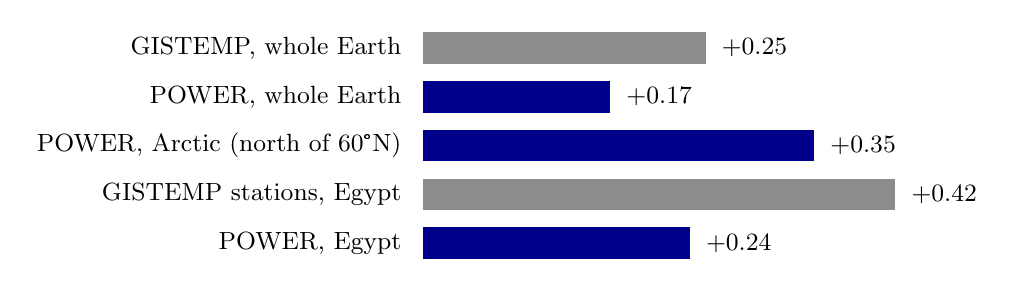
\begin{tikzpicture}
\node[anchor=east, font=\small] at (-0.15,0.20) {GISTEMP, whole Earth};\fill[black!45] (0,0.00) rectangle (3.59,0.40);\node[anchor=west, font=\small] at (3.67,0.20) {$+0.25$};
\node[anchor=east, font=\small] at (-0.15,-0.42) {POWER, whole Earth};\fill[blue!55!black] (0,-0.62) rectangle (2.38,-0.22);\node[anchor=west, font=\small] at (2.46,-0.42) {$+0.17$};
\node[anchor=east, font=\small] at (-0.15,-1.04) {POWER, Arctic (north of 60\textdegree{}N)};\fill[blue!55!black] (0,-1.24) rectangle (4.97,-0.84);\node[anchor=west, font=\small] at (5.05,-1.04) {$+0.35$};
\node[anchor=east, font=\small] at (-0.15,-1.66) {GISTEMP stations, Egypt};\fill[black!45] (0,-1.86) rectangle (6.00,-1.46);\node[anchor=west, font=\small] at (6.08,-1.66) {$+0.42$};
\node[anchor=east, font=\small] at (-0.15,-2.28) {POWER, Egypt};\fill[blue!55!black] (0,-2.48) rectangle (3.39,-2.08);\node[anchor=west, font=\small] at (3.47,-2.28) {$+0.24$};
\end{tikzpicture}
\caption{Trends in air temperature, 2001--2025, \degC{} per decade, all computed with our engine. Grey: NASA GISTEMP (weather stations); blue: NASA POWER (the data used in the app).}\label{fig:bars}
\end{figure}

Over Egypt the difference between the two records is noticeable. The stations warm by $+0.42$\degC{} per decade and the trend is proven in 30 of 32 station areas; POWER warms by $+0.24$\degC{} per decade and proves it in 12. In other words POWER is conservative here, and many cells read ``not proven'' that the stations would call warming. Rather than hide this, the app shows the station trend next to every air temperature answer.

\subsection{Egypt and Sudan}
Figure~\ref{fig:maps} shows the air temperature trend for every grid cell of Egypt and Sudan. In Egypt 85 of 324 cells show proven warming and none show cooling (median trend $+0.23$\degC{} per decade); the proven cells follow the Nile valley, the Delta and the Red Sea coast. In Cairo the yearly mean rose by $+0.29$\degC{} per decade (95\% range $+0.03$ to $+0.51$, moderate evidence, $p=0.027$), while the surrounding station record shows $+0.48$\degC{} per decade with strong evidence (Figure~\ref{fig:cairo}).

Sudan illustrates the challenge's point about opposite trends. Air temperature has fallen with proven evidence in 238 cells in the south and risen in 26 cells in the north, inside one country and over the same years. We do not attribute a cause here, which would need the rain and soil records alongside, but this is exactly the kind of contrast that a single national average would hide.

\begin{figure}[h]\centering
\begin{minipage}[b]{0.43\linewidth}\centering
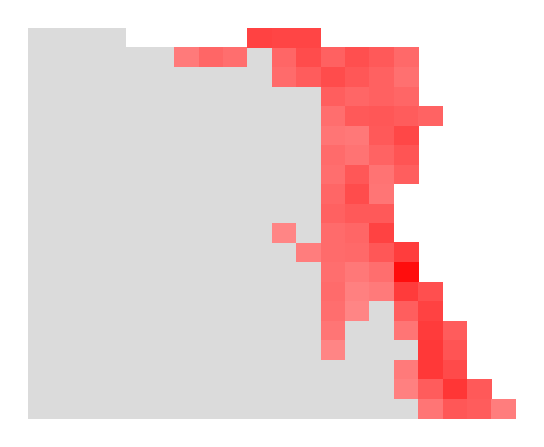
\begin{tikzpicture}
\fill[black!14] (0.000,0.000) rectangle ++(0.314,0.252);
\fill[black!14] (0.310,0.000) rectangle ++(0.314,0.252);
\fill[black!14] (0.620,0.000) rectangle ++(0.314,0.252);
\fill[black!14] (0.930,0.000) rectangle ++(0.314,0.252);
\fill[black!14] (1.240,0.000) rectangle ++(0.314,0.252);
\fill[black!14] (1.550,0.000) rectangle ++(0.314,0.252);
\fill[black!14] (1.860,0.000) rectangle ++(0.314,0.252);
\fill[black!14] (2.170,0.000) rectangle ++(0.314,0.252);
\fill[black!14] (2.480,0.000) rectangle ++(0.314,0.252);
\fill[black!14] (2.790,0.000) rectangle ++(0.314,0.252);
\fill[black!14] (3.100,0.000) rectangle ++(0.314,0.252);
\fill[black!14] (3.410,0.000) rectangle ++(0.314,0.252);
\fill[black!14] (3.720,0.000) rectangle ++(0.314,0.252);
\fill[black!14] (4.030,0.000) rectangle ++(0.314,0.252);
\fill[black!14] (4.340,0.000) rectangle ++(0.314,0.252);
\fill[black!14] (4.650,0.000) rectangle ++(0.314,0.252);
\fill[red!54!white] (4.960,0.000) rectangle ++(0.314,0.252);
\fill[red!66!white] (5.270,0.000) rectangle ++(0.314,0.252);
\fill[red!64!white] (5.580,0.000) rectangle ++(0.314,0.252);
\fill[red!51!white] (5.890,0.000) rectangle ++(0.314,0.252);
\fill[black!14] (0.000,0.248) rectangle ++(0.314,0.252);
\fill[black!14] (0.310,0.248) rectangle ++(0.314,0.252);
\fill[black!14] (0.620,0.248) rectangle ++(0.314,0.252);
\fill[black!14] (0.930,0.248) rectangle ++(0.314,0.252);
\fill[black!14] (1.240,0.248) rectangle ++(0.314,0.252);
\fill[black!14] (1.550,0.248) rectangle ++(0.314,0.252);
\fill[black!14] (1.860,0.248) rectangle ++(0.314,0.252);
\fill[black!14] (2.170,0.248) rectangle ++(0.314,0.252);
\fill[black!14] (2.480,0.248) rectangle ++(0.314,0.252);
\fill[black!14] (2.790,0.248) rectangle ++(0.314,0.252);
\fill[black!14] (3.100,0.248) rectangle ++(0.314,0.252);
\fill[black!14] (3.410,0.248) rectangle ++(0.314,0.252);
\fill[black!14] (3.720,0.248) rectangle ++(0.314,0.252);
\fill[black!14] (4.030,0.248) rectangle ++(0.314,0.252);
\fill[black!14] (4.340,0.248) rectangle ++(0.314,0.252);
\fill[red!50!white] (4.650,0.248) rectangle ++(0.314,0.252);
\fill[red!64!white] (4.960,0.248) rectangle ++(0.314,0.252);
\fill[red!79!white] (5.270,0.248) rectangle ++(0.314,0.252);
\fill[red!65!white] (5.580,0.248) rectangle ++(0.314,0.252);
\fill[black!14] (0.000,0.496) rectangle ++(0.314,0.252);
\fill[black!14] (0.310,0.496) rectangle ++(0.314,0.252);
\fill[black!14] (0.620,0.496) rectangle ++(0.314,0.252);
\fill[black!14] (0.930,0.496) rectangle ++(0.314,0.252);
\fill[black!14] (1.240,0.496) rectangle ++(0.314,0.252);
\fill[black!14] (1.550,0.496) rectangle ++(0.314,0.252);
\fill[black!14] (1.860,0.496) rectangle ++(0.314,0.252);
\fill[black!14] (2.170,0.496) rectangle ++(0.314,0.252);
\fill[black!14] (2.480,0.496) rectangle ++(0.314,0.252);
\fill[black!14] (2.790,0.496) rectangle ++(0.314,0.252);
\fill[black!14] (3.100,0.496) rectangle ++(0.314,0.252);
\fill[black!14] (3.410,0.496) rectangle ++(0.314,0.252);
\fill[black!14] (3.720,0.496) rectangle ++(0.314,0.252);
\fill[black!14] (4.030,0.496) rectangle ++(0.314,0.252);
\fill[black!14] (4.340,0.496) rectangle ++(0.314,0.252);
\fill[red!52!white] (4.650,0.496) rectangle ++(0.314,0.252);
\fill[red!78!white] (4.960,0.496) rectangle ++(0.314,0.252);
\fill[red!71!white] (5.270,0.496) rectangle ++(0.314,0.252);
\fill[black!14] (0.000,0.744) rectangle ++(0.314,0.252);
\fill[black!14] (0.310,0.744) rectangle ++(0.314,0.252);
\fill[black!14] (0.620,0.744) rectangle ++(0.314,0.252);
\fill[black!14] (0.930,0.744) rectangle ++(0.314,0.252);
\fill[black!14] (1.240,0.744) rectangle ++(0.314,0.252);
\fill[black!14] (1.550,0.744) rectangle ++(0.314,0.252);
\fill[black!14] (1.860,0.744) rectangle ++(0.314,0.252);
\fill[black!14] (2.170,0.744) rectangle ++(0.314,0.252);
\fill[black!14] (2.480,0.744) rectangle ++(0.314,0.252);
\fill[black!14] (2.790,0.744) rectangle ++(0.314,0.252);
\fill[black!14] (3.100,0.744) rectangle ++(0.314,0.252);
\fill[black!14] (3.410,0.744) rectangle ++(0.314,0.252);
\fill[red!48!white] (3.720,0.744) rectangle ++(0.314,0.252);
\fill[black!14] (4.030,0.744) rectangle ++(0.314,0.252);
\fill[black!14] (4.340,0.744) rectangle ++(0.314,0.252);
\fill[black!14] (4.650,0.744) rectangle ++(0.314,0.252);
\fill[red!78!white] (4.960,0.744) rectangle ++(0.314,0.252);
\fill[red!67!white] (5.270,0.744) rectangle ++(0.314,0.252);
\fill[black!14] (0.000,0.992) rectangle ++(0.314,0.252);
\fill[black!14] (0.310,0.992) rectangle ++(0.314,0.252);
\fill[black!14] (0.620,0.992) rectangle ++(0.314,0.252);
\fill[black!14] (0.930,0.992) rectangle ++(0.314,0.252);
\fill[black!14] (1.240,0.992) rectangle ++(0.314,0.252);
\fill[black!14] (1.550,0.992) rectangle ++(0.314,0.252);
\fill[black!14] (1.860,0.992) rectangle ++(0.314,0.252);
\fill[black!14] (2.170,0.992) rectangle ++(0.314,0.252);
\fill[black!14] (2.480,0.992) rectangle ++(0.314,0.252);
\fill[black!14] (2.790,0.992) rectangle ++(0.314,0.252);
\fill[black!14] (3.100,0.992) rectangle ++(0.314,0.252);
\fill[black!14] (3.410,0.992) rectangle ++(0.314,0.252);
\fill[red!54!white] (3.720,0.992) rectangle ++(0.314,0.252);
\fill[black!14] (4.030,0.992) rectangle ++(0.314,0.252);
\fill[black!14] (4.340,0.992) rectangle ++(0.314,0.252);
\fill[red!54!white] (4.650,0.992) rectangle ++(0.314,0.252);
\fill[red!77!white] (4.960,0.992) rectangle ++(0.314,0.252);
\fill[red!64!white] (5.270,0.992) rectangle ++(0.314,0.252);
\fill[black!14] (0.000,1.240) rectangle ++(0.314,0.252);
\fill[black!14] (0.310,1.240) rectangle ++(0.314,0.252);
\fill[black!14] (0.620,1.240) rectangle ++(0.314,0.252);
\fill[black!14] (0.930,1.240) rectangle ++(0.314,0.252);
\fill[black!14] (1.240,1.240) rectangle ++(0.314,0.252);
\fill[black!14] (1.550,1.240) rectangle ++(0.314,0.252);
\fill[black!14] (1.860,1.240) rectangle ++(0.314,0.252);
\fill[black!14] (2.170,1.240) rectangle ++(0.314,0.252);
\fill[black!14] (2.480,1.240) rectangle ++(0.314,0.252);
\fill[black!14] (2.790,1.240) rectangle ++(0.314,0.252);
\fill[black!14] (3.100,1.240) rectangle ++(0.314,0.252);
\fill[black!14] (3.410,1.240) rectangle ++(0.314,0.252);
\fill[red!57!white] (3.720,1.240) rectangle ++(0.314,0.252);
\fill[red!48!white] (4.030,1.240) rectangle ++(0.314,0.252);
\fill[black!14] (4.340,1.240) rectangle ++(0.314,0.252);
\fill[red!63!white] (4.650,1.240) rectangle ++(0.314,0.252);
\fill[red!74!white] (4.960,1.240) rectangle ++(0.314,0.252);
\fill[black!14] (0.000,1.488) rectangle ++(0.314,0.252);
\fill[black!14] (0.310,1.488) rectangle ++(0.314,0.252);
\fill[black!14] (0.620,1.488) rectangle ++(0.314,0.252);
\fill[black!14] (0.930,1.488) rectangle ++(0.314,0.252);
\fill[black!14] (1.240,1.488) rectangle ++(0.314,0.252);
\fill[black!14] (1.550,1.488) rectangle ++(0.314,0.252);
\fill[black!14] (1.860,1.488) rectangle ++(0.314,0.252);
\fill[black!14] (2.170,1.488) rectangle ++(0.314,0.252);
\fill[black!14] (2.480,1.488) rectangle ++(0.314,0.252);
\fill[black!14] (2.790,1.488) rectangle ++(0.314,0.252);
\fill[black!14] (3.100,1.488) rectangle ++(0.314,0.252);
\fill[black!14] (3.410,1.488) rectangle ++(0.314,0.252);
\fill[red!58!white] (3.720,1.488) rectangle ++(0.314,0.252);
\fill[red!50!white] (4.030,1.488) rectangle ++(0.314,0.252);
\fill[red!52!white] (4.340,1.488) rectangle ++(0.314,0.252);
\fill[red!77!white] (4.650,1.488) rectangle ++(0.314,0.252);
\fill[red!69!white] (4.960,1.488) rectangle ++(0.314,0.252);
\fill[black!14] (0.000,1.736) rectangle ++(0.314,0.252);
\fill[black!14] (0.310,1.736) rectangle ++(0.314,0.252);
\fill[black!14] (0.620,1.736) rectangle ++(0.314,0.252);
\fill[black!14] (0.930,1.736) rectangle ++(0.314,0.252);
\fill[black!14] (1.240,1.736) rectangle ++(0.314,0.252);
\fill[black!14] (1.550,1.736) rectangle ++(0.314,0.252);
\fill[black!14] (1.860,1.736) rectangle ++(0.314,0.252);
\fill[black!14] (2.170,1.736) rectangle ++(0.314,0.252);
\fill[black!14] (2.480,1.736) rectangle ++(0.314,0.252);
\fill[black!14] (2.790,1.736) rectangle ++(0.314,0.252);
\fill[black!14] (3.100,1.736) rectangle ++(0.314,0.252);
\fill[black!14] (3.410,1.736) rectangle ++(0.314,0.252);
\fill[red!57!white] (3.720,1.736) rectangle ++(0.314,0.252);
\fill[red!53!white] (4.030,1.736) rectangle ++(0.314,0.252);
\fill[red!57!white] (4.340,1.736) rectangle ++(0.314,0.252);
\fill[red!95!white] (4.650,1.736) rectangle ++(0.314,0.252);
\fill[black!14] (0.000,1.984) rectangle ++(0.314,0.252);
\fill[black!14] (0.310,1.984) rectangle ++(0.314,0.252);
\fill[black!14] (0.620,1.984) rectangle ++(0.314,0.252);
\fill[black!14] (0.930,1.984) rectangle ++(0.314,0.252);
\fill[black!14] (1.240,1.984) rectangle ++(0.314,0.252);
\fill[black!14] (1.550,1.984) rectangle ++(0.314,0.252);
\fill[black!14] (1.860,1.984) rectangle ++(0.314,0.252);
\fill[black!14] (2.170,1.984) rectangle ++(0.314,0.252);
\fill[black!14] (2.480,1.984) rectangle ++(0.314,0.252);
\fill[black!14] (2.790,1.984) rectangle ++(0.314,0.252);
\fill[black!14] (3.100,1.984) rectangle ++(0.314,0.252);
\fill[red!51!white] (3.410,1.984) rectangle ++(0.314,0.252);
\fill[red!58!white] (3.720,1.984) rectangle ++(0.314,0.252);
\fill[red!59!white] (4.030,1.984) rectangle ++(0.314,0.252);
\fill[red!66!white] (4.340,1.984) rectangle ++(0.314,0.252);
\fill[red!76!white] (4.650,1.984) rectangle ++(0.314,0.252);
\fill[black!14] (0.000,2.232) rectangle ++(0.314,0.252);
\fill[black!14] (0.310,2.232) rectangle ++(0.314,0.252);
\fill[black!14] (0.620,2.232) rectangle ++(0.314,0.252);
\fill[black!14] (0.930,2.232) rectangle ++(0.314,0.252);
\fill[black!14] (1.240,2.232) rectangle ++(0.314,0.252);
\fill[black!14] (1.550,2.232) rectangle ++(0.314,0.252);
\fill[black!14] (1.860,2.232) rectangle ++(0.314,0.252);
\fill[black!14] (2.170,2.232) rectangle ++(0.314,0.252);
\fill[black!14] (2.480,2.232) rectangle ++(0.314,0.252);
\fill[black!14] (2.790,2.232) rectangle ++(0.314,0.252);
\fill[red!48!white] (3.100,2.232) rectangle ++(0.314,0.252);
\fill[black!14] (3.410,2.232) rectangle ++(0.314,0.252);
\fill[red!58!white] (3.720,2.232) rectangle ++(0.314,0.252);
\fill[red!60!white] (4.030,2.232) rectangle ++(0.314,0.252);
\fill[red!74!white] (4.340,2.232) rectangle ++(0.314,0.252);
\fill[black!14] (0.000,2.480) rectangle ++(0.314,0.252);
\fill[black!14] (0.310,2.480) rectangle ++(0.314,0.252);
\fill[black!14] (0.620,2.480) rectangle ++(0.314,0.252);
\fill[black!14] (0.930,2.480) rectangle ++(0.314,0.252);
\fill[black!14] (1.240,2.480) rectangle ++(0.314,0.252);
\fill[black!14] (1.550,2.480) rectangle ++(0.314,0.252);
\fill[black!14] (1.860,2.480) rectangle ++(0.314,0.252);
\fill[black!14] (2.170,2.480) rectangle ++(0.314,0.252);
\fill[black!14] (2.480,2.480) rectangle ++(0.314,0.252);
\fill[black!14] (2.790,2.480) rectangle ++(0.314,0.252);
\fill[black!14] (3.100,2.480) rectangle ++(0.314,0.252);
\fill[black!14] (3.410,2.480) rectangle ++(0.314,0.252);
\fill[red!62!white] (3.720,2.480) rectangle ++(0.314,0.252);
\fill[red!65!white] (4.030,2.480) rectangle ++(0.314,0.252);
\fill[red!65!white] (4.340,2.480) rectangle ++(0.314,0.252);
\fill[black!14] (0.000,2.728) rectangle ++(0.314,0.252);
\fill[black!14] (0.310,2.728) rectangle ++(0.314,0.252);
\fill[black!14] (0.620,2.728) rectangle ++(0.314,0.252);
\fill[black!14] (0.930,2.728) rectangle ++(0.314,0.252);
\fill[black!14] (1.240,2.728) rectangle ++(0.314,0.252);
\fill[black!14] (1.550,2.728) rectangle ++(0.314,0.252);
\fill[black!14] (1.860,2.728) rectangle ++(0.314,0.252);
\fill[black!14] (2.170,2.728) rectangle ++(0.314,0.252);
\fill[black!14] (2.480,2.728) rectangle ++(0.314,0.252);
\fill[black!14] (2.790,2.728) rectangle ++(0.314,0.252);
\fill[black!14] (3.100,2.728) rectangle ++(0.314,0.252);
\fill[black!14] (3.410,2.728) rectangle ++(0.314,0.252);
\fill[red!60!white] (3.720,2.728) rectangle ++(0.314,0.252);
\fill[red!70!white] (4.030,2.728) rectangle ++(0.314,0.252);
\fill[red!54!white] (4.340,2.728) rectangle ++(0.314,0.252);
\fill[black!14] (0.000,2.976) rectangle ++(0.314,0.252);
\fill[black!14] (0.310,2.976) rectangle ++(0.314,0.252);
\fill[black!14] (0.620,2.976) rectangle ++(0.314,0.252);
\fill[black!14] (0.930,2.976) rectangle ++(0.314,0.252);
\fill[black!14] (1.240,2.976) rectangle ++(0.314,0.252);
\fill[black!14] (1.550,2.976) rectangle ++(0.314,0.252);
\fill[black!14] (1.860,2.976) rectangle ++(0.314,0.252);
\fill[black!14] (2.170,2.976) rectangle ++(0.314,0.252);
\fill[black!14] (2.480,2.976) rectangle ++(0.314,0.252);
\fill[black!14] (2.790,2.976) rectangle ++(0.314,0.252);
\fill[black!14] (3.100,2.976) rectangle ++(0.314,0.252);
\fill[black!14] (3.410,2.976) rectangle ++(0.314,0.252);
\fill[red!57!white] (3.720,2.976) rectangle ++(0.314,0.252);
\fill[red!66!white] (4.030,2.976) rectangle ++(0.314,0.252);
\fill[red!55!white] (4.340,2.976) rectangle ++(0.314,0.252);
\fill[red!63!white] (4.650,2.976) rectangle ++(0.314,0.252);
\fill[black!14] (0.000,3.224) rectangle ++(0.314,0.252);
\fill[black!14] (0.310,3.224) rectangle ++(0.314,0.252);
\fill[black!14] (0.620,3.224) rectangle ++(0.314,0.252);
\fill[black!14] (0.930,3.224) rectangle ++(0.314,0.252);
\fill[black!14] (1.240,3.224) rectangle ++(0.314,0.252);
\fill[black!14] (1.550,3.224) rectangle ++(0.314,0.252);
\fill[black!14] (1.860,3.224) rectangle ++(0.314,0.252);
\fill[black!14] (2.170,3.224) rectangle ++(0.314,0.252);
\fill[black!14] (2.480,3.224) rectangle ++(0.314,0.252);
\fill[black!14] (2.790,3.224) rectangle ++(0.314,0.252);
\fill[black!14] (3.100,3.224) rectangle ++(0.314,0.252);
\fill[black!14] (3.410,3.224) rectangle ++(0.314,0.252);
\fill[red!58!white] (3.720,3.224) rectangle ++(0.314,0.252);
\fill[red!55!white] (4.030,3.224) rectangle ++(0.314,0.252);
\fill[red!61!white] (4.340,3.224) rectangle ++(0.314,0.252);
\fill[red!67!white] (4.650,3.224) rectangle ++(0.314,0.252);
\fill[black!14] (0.000,3.472) rectangle ++(0.314,0.252);
\fill[black!14] (0.310,3.472) rectangle ++(0.314,0.252);
\fill[black!14] (0.620,3.472) rectangle ++(0.314,0.252);
\fill[black!14] (0.930,3.472) rectangle ++(0.314,0.252);
\fill[black!14] (1.240,3.472) rectangle ++(0.314,0.252);
\fill[black!14] (1.550,3.472) rectangle ++(0.314,0.252);
\fill[black!14] (1.860,3.472) rectangle ++(0.314,0.252);
\fill[black!14] (2.170,3.472) rectangle ++(0.314,0.252);
\fill[black!14] (2.480,3.472) rectangle ++(0.314,0.252);
\fill[black!14] (2.790,3.472) rectangle ++(0.314,0.252);
\fill[black!14] (3.100,3.472) rectangle ++(0.314,0.252);
\fill[black!14] (3.410,3.472) rectangle ++(0.314,0.252);
\fill[red!54!white] (3.720,3.472) rectangle ++(0.314,0.252);
\fill[red!53!white] (4.030,3.472) rectangle ++(0.314,0.252);
\fill[red!65!white] (4.340,3.472) rectangle ++(0.314,0.252);
\fill[red!72!white] (4.650,3.472) rectangle ++(0.314,0.252);
\fill[black!14] (0.000,3.720) rectangle ++(0.314,0.252);
\fill[black!14] (0.310,3.720) rectangle ++(0.314,0.252);
\fill[black!14] (0.620,3.720) rectangle ++(0.314,0.252);
\fill[black!14] (0.930,3.720) rectangle ++(0.314,0.252);
\fill[black!14] (1.240,3.720) rectangle ++(0.314,0.252);
\fill[black!14] (1.550,3.720) rectangle ++(0.314,0.252);
\fill[black!14] (1.860,3.720) rectangle ++(0.314,0.252);
\fill[black!14] (2.170,3.720) rectangle ++(0.314,0.252);
\fill[black!14] (2.480,3.720) rectangle ++(0.314,0.252);
\fill[black!14] (2.790,3.720) rectangle ++(0.314,0.252);
\fill[black!14] (3.100,3.720) rectangle ++(0.314,0.252);
\fill[black!14] (3.410,3.720) rectangle ++(0.314,0.252);
\fill[red!57!white] (3.720,3.720) rectangle ++(0.314,0.252);
\fill[red!65!white] (4.030,3.720) rectangle ++(0.314,0.252);
\fill[red!66!white] (4.340,3.720) rectangle ++(0.314,0.252);
\fill[red!64!white] (4.650,3.720) rectangle ++(0.314,0.252);
\fill[red!61!white] (4.960,3.720) rectangle ++(0.314,0.252);
\fill[black!14] (0.000,3.968) rectangle ++(0.314,0.252);
\fill[black!14] (0.310,3.968) rectangle ++(0.314,0.252);
\fill[black!14] (0.620,3.968) rectangle ++(0.314,0.252);
\fill[black!14] (0.930,3.968) rectangle ++(0.314,0.252);
\fill[black!14] (1.240,3.968) rectangle ++(0.314,0.252);
\fill[black!14] (1.550,3.968) rectangle ++(0.314,0.252);
\fill[black!14] (1.860,3.968) rectangle ++(0.314,0.252);
\fill[black!14] (2.170,3.968) rectangle ++(0.314,0.252);
\fill[black!14] (2.480,3.968) rectangle ++(0.314,0.252);
\fill[black!14] (2.790,3.968) rectangle ++(0.314,0.252);
\fill[black!14] (3.100,3.968) rectangle ++(0.314,0.252);
\fill[black!14] (3.410,3.968) rectangle ++(0.314,0.252);
\fill[red!63!white] (3.720,3.968) rectangle ++(0.314,0.252);
\fill[red!60!white] (4.030,3.968) rectangle ++(0.314,0.252);
\fill[red!62!white] (4.340,3.968) rectangle ++(0.314,0.252);
\fill[red!60!white] (4.650,3.968) rectangle ++(0.314,0.252);
\fill[black!14] (0.000,4.216) rectangle ++(0.314,0.252);
\fill[black!14] (0.310,4.216) rectangle ++(0.314,0.252);
\fill[black!14] (0.620,4.216) rectangle ++(0.314,0.252);
\fill[black!14] (0.930,4.216) rectangle ++(0.314,0.252);
\fill[black!14] (1.240,4.216) rectangle ++(0.314,0.252);
\fill[black!14] (1.550,4.216) rectangle ++(0.314,0.252);
\fill[black!14] (1.860,4.216) rectangle ++(0.314,0.252);
\fill[black!14] (2.170,4.216) rectangle ++(0.314,0.252);
\fill[black!14] (2.480,4.216) rectangle ++(0.314,0.252);
\fill[black!14] (2.790,4.216) rectangle ++(0.314,0.252);
\fill[red!58!white] (3.100,4.216) rectangle ++(0.314,0.252);
\fill[red!64!white] (3.410,4.216) rectangle ++(0.314,0.252);
\fill[red!70!white] (3.720,4.216) rectangle ++(0.314,0.252);
\fill[red!66!white] (4.030,4.216) rectangle ++(0.314,0.252);
\fill[red!62!white] (4.340,4.216) rectangle ++(0.314,0.252);
\fill[red!56!white] (4.650,4.216) rectangle ++(0.314,0.252);
\fill[black!14] (0.000,4.464) rectangle ++(0.314,0.252);
\fill[black!14] (0.310,4.464) rectangle ++(0.314,0.252);
\fill[black!14] (0.620,4.464) rectangle ++(0.314,0.252);
\fill[black!14] (0.930,4.464) rectangle ++(0.314,0.252);
\fill[black!14] (1.240,4.464) rectangle ++(0.314,0.252);
\fill[black!14] (1.550,4.464) rectangle ++(0.314,0.252);
\fill[red!52!white] (1.860,4.464) rectangle ++(0.314,0.252);
\fill[red!60!white] (2.170,4.464) rectangle ++(0.314,0.252);
\fill[red!57!white] (2.480,4.464) rectangle ++(0.314,0.252);
\fill[black!14] (2.790,4.464) rectangle ++(0.314,0.252);
\fill[red!60!white] (3.100,4.464) rectangle ++(0.314,0.252);
\fill[red!70!white] (3.410,4.464) rectangle ++(0.314,0.252);
\fill[red!62!white] (3.720,4.464) rectangle ++(0.314,0.252);
\fill[red!69!white] (4.030,4.464) rectangle ++(0.314,0.252);
\fill[red!65!white] (4.340,4.464) rectangle ++(0.314,0.252);
\fill[red!59!white] (4.650,4.464) rectangle ++(0.314,0.252);
\fill[black!14] (0.000,4.712) rectangle ++(0.314,0.252);
\fill[black!14] (0.310,4.712) rectangle ++(0.314,0.252);
\fill[black!14] (0.620,4.712) rectangle ++(0.314,0.252);
\fill[black!14] (0.930,4.712) rectangle ++(0.314,0.252);
\fill[red!74!white] (2.790,4.712) rectangle ++(0.314,0.252);
\fill[red!73!white] (3.100,4.712) rectangle ++(0.314,0.252);
\fill[red!73!white] (3.410,4.712) rectangle ++(0.314,0.252);
\end{tikzpicture}\\[3pt]\small (a) Egypt
\end{minipage}\hfill
\begin{minipage}[b]{0.53\linewidth}\centering
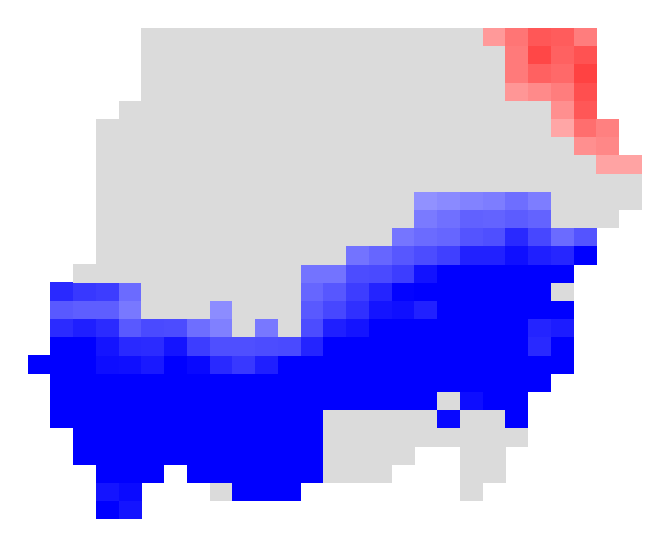
\begin{tikzpicture}
\fill[blue!100!white] (0.867,0.000) rectangle ++(0.293,0.235);
\fill[blue!92!white] (1.156,0.000) rectangle ++(0.293,0.235);
\fill[blue!92!white] (0.867,0.231) rectangle ++(0.293,0.235);
\fill[blue!96!white] (1.156,0.231) rectangle ++(0.293,0.235);
\fill[black!14] (2.311,0.231) rectangle ++(0.293,0.235);
\fill[blue!100!white] (2.600,0.231) rectangle ++(0.293,0.235);
\fill[blue!100!white] (2.889,0.231) rectangle ++(0.293,0.235);
\fill[blue!100!white] (3.178,0.231) rectangle ++(0.293,0.235);
\fill[black!14] (5.489,0.231) rectangle ++(0.293,0.235);
\fill[blue!100!white] (0.867,0.462) rectangle ++(0.293,0.235);
\fill[blue!100!white] (1.156,0.462) rectangle ++(0.293,0.235);
\fill[blue!100!white] (1.444,0.462) rectangle ++(0.293,0.235);
\fill[blue!100!white] (2.022,0.462) rectangle ++(0.293,0.235);
\fill[blue!100!white] (2.311,0.462) rectangle ++(0.293,0.235);
\fill[blue!100!white] (2.600,0.462) rectangle ++(0.293,0.235);
\fill[blue!100!white] (2.889,0.462) rectangle ++(0.293,0.235);
\fill[blue!100!white] (3.178,0.462) rectangle ++(0.293,0.235);
\fill[blue!100!white] (3.467,0.462) rectangle ++(0.293,0.235);
\fill[black!14] (3.756,0.462) rectangle ++(0.293,0.235);
\fill[black!14] (4.044,0.462) rectangle ++(0.293,0.235);
\fill[black!14] (4.333,0.462) rectangle ++(0.293,0.235);
\fill[black!14] (5.489,0.462) rectangle ++(0.293,0.235);
\fill[black!14] (5.778,0.462) rectangle ++(0.293,0.235);
\fill[blue!100!white] (0.578,0.693) rectangle ++(0.293,0.235);
\fill[blue!100!white] (0.867,0.693) rectangle ++(0.293,0.235);
\fill[blue!100!white] (1.156,0.693) rectangle ++(0.293,0.235);
\fill[blue!100!white] (1.444,0.693) rectangle ++(0.293,0.235);
\fill[blue!100!white] (1.733,0.693) rectangle ++(0.293,0.235);
\fill[blue!100!white] (2.022,0.693) rectangle ++(0.293,0.235);
\fill[blue!100!white] (2.311,0.693) rectangle ++(0.293,0.235);
\fill[blue!100!white] (2.600,0.693) rectangle ++(0.293,0.235);
\fill[blue!100!white] (2.889,0.693) rectangle ++(0.293,0.235);
\fill[blue!100!white] (3.178,0.693) rectangle ++(0.293,0.235);
\fill[blue!100!white] (3.467,0.693) rectangle ++(0.293,0.235);
\fill[black!14] (3.756,0.693) rectangle ++(0.293,0.235);
\fill[black!14] (4.044,0.693) rectangle ++(0.293,0.235);
\fill[black!14] (4.333,0.693) rectangle ++(0.293,0.235);
\fill[black!14] (4.622,0.693) rectangle ++(0.293,0.235);
\fill[black!14] (5.489,0.693) rectangle ++(0.293,0.235);
\fill[black!14] (5.778,0.693) rectangle ++(0.293,0.235);
\fill[blue!100!white] (0.578,0.924) rectangle ++(0.293,0.235);
\fill[blue!100!white] (0.867,0.924) rectangle ++(0.293,0.235);
\fill[blue!100!white] (1.156,0.924) rectangle ++(0.293,0.235);
\fill[blue!100!white] (1.444,0.924) rectangle ++(0.293,0.235);
\fill[blue!100!white] (1.733,0.924) rectangle ++(0.293,0.235);
\fill[blue!100!white] (2.022,0.924) rectangle ++(0.293,0.235);
\fill[blue!100!white] (2.311,0.924) rectangle ++(0.293,0.235);
\fill[blue!100!white] (2.600,0.924) rectangle ++(0.293,0.235);
\fill[blue!100!white] (2.889,0.924) rectangle ++(0.293,0.235);
\fill[blue!100!white] (3.178,0.924) rectangle ++(0.293,0.235);
\fill[blue!100!white] (3.467,0.924) rectangle ++(0.293,0.235);
\fill[black!14] (3.756,0.924) rectangle ++(0.293,0.235);
\fill[black!14] (4.044,0.924) rectangle ++(0.293,0.235);
\fill[black!14] (4.333,0.924) rectangle ++(0.293,0.235);
\fill[black!14] (4.622,0.924) rectangle ++(0.293,0.235);
\fill[black!14] (4.911,0.924) rectangle ++(0.293,0.235);
\fill[black!14] (5.200,0.924) rectangle ++(0.293,0.235);
\fill[black!14] (5.489,0.924) rectangle ++(0.293,0.235);
\fill[black!14] (5.778,0.924) rectangle ++(0.293,0.235);
\fill[black!14] (6.067,0.924) rectangle ++(0.293,0.235);
\fill[blue!100!white] (0.289,1.156) rectangle ++(0.293,0.235);
\fill[blue!100!white] (0.578,1.156) rectangle ++(0.293,0.235);
\fill[blue!100!white] (0.867,1.156) rectangle ++(0.293,0.235);
\fill[blue!100!white] (1.156,1.156) rectangle ++(0.293,0.235);
\fill[blue!100!white] (1.444,1.156) rectangle ++(0.293,0.235);
\fill[blue!100!white] (1.733,1.156) rectangle ++(0.293,0.235);
\fill[blue!100!white] (2.022,1.156) rectangle ++(0.293,0.235);
\fill[blue!100!white] (2.311,1.156) rectangle ++(0.293,0.235);
\fill[blue!100!white] (2.600,1.156) rectangle ++(0.293,0.235);
\fill[blue!100!white] (2.889,1.156) rectangle ++(0.293,0.235);
\fill[blue!100!white] (3.178,1.156) rectangle ++(0.293,0.235);
\fill[blue!100!white] (3.467,1.156) rectangle ++(0.293,0.235);
\fill[black!14] (3.756,1.156) rectangle ++(0.293,0.235);
\fill[black!14] (4.044,1.156) rectangle ++(0.293,0.235);
\fill[black!14] (4.333,1.156) rectangle ++(0.293,0.235);
\fill[black!14] (4.622,1.156) rectangle ++(0.293,0.235);
\fill[black!14] (4.911,1.156) rectangle ++(0.293,0.235);
\fill[blue!97!white] (5.200,1.156) rectangle ++(0.293,0.235);
\fill[black!14] (5.489,1.156) rectangle ++(0.293,0.235);
\fill[black!14] (5.778,1.156) rectangle ++(0.293,0.235);
\fill[blue!100!white] (6.067,1.156) rectangle ++(0.293,0.235);
\fill[blue!100!white] (0.289,1.387) rectangle ++(0.293,0.235);
\fill[blue!100!white] (0.578,1.387) rectangle ++(0.293,0.235);
\fill[blue!100!white] (0.867,1.387) rectangle ++(0.293,0.235);
\fill[blue!100!white] (1.156,1.387) rectangle ++(0.293,0.235);
\fill[blue!100!white] (1.444,1.387) rectangle ++(0.293,0.235);
\fill[blue!100!white] (1.733,1.387) rectangle ++(0.293,0.235);
\fill[blue!100!white] (2.022,1.387) rectangle ++(0.293,0.235);
\fill[blue!100!white] (2.311,1.387) rectangle ++(0.293,0.235);
\fill[blue!100!white] (2.600,1.387) rectangle ++(0.293,0.235);
\fill[blue!100!white] (2.889,1.387) rectangle ++(0.293,0.235);
\fill[blue!100!white] (3.178,1.387) rectangle ++(0.293,0.235);
\fill[blue!100!white] (3.467,1.387) rectangle ++(0.293,0.235);
\fill[blue!100!white] (3.756,1.387) rectangle ++(0.293,0.235);
\fill[blue!100!white] (4.044,1.387) rectangle ++(0.293,0.235);
\fill[blue!100!white] (4.333,1.387) rectangle ++(0.293,0.235);
\fill[blue!100!white] (4.622,1.387) rectangle ++(0.293,0.235);
\fill[blue!100!white] (4.911,1.387) rectangle ++(0.293,0.235);
\fill[black!14] (5.200,1.387) rectangle ++(0.293,0.235);
\fill[blue!95!white] (5.489,1.387) rectangle ++(0.293,0.235);
\fill[blue!100!white] (5.778,1.387) rectangle ++(0.293,0.235);
\fill[blue!100!white] (6.067,1.387) rectangle ++(0.293,0.235);
\fill[blue!100!white] (0.289,1.618) rectangle ++(0.293,0.235);
\fill[blue!100!white] (0.578,1.618) rectangle ++(0.293,0.235);
\fill[blue!100!white] (0.867,1.618) rectangle ++(0.293,0.235);
\fill[blue!100!white] (1.156,1.618) rectangle ++(0.293,0.235);
\fill[blue!100!white] (1.444,1.618) rectangle ++(0.293,0.235);
\fill[blue!100!white] (1.733,1.618) rectangle ++(0.293,0.235);
\fill[blue!100!white] (2.022,1.618) rectangle ++(0.293,0.235);
\fill[blue!100!white] (2.311,1.618) rectangle ++(0.293,0.235);
\fill[blue!100!white] (2.600,1.618) rectangle ++(0.293,0.235);
\fill[blue!100!white] (2.889,1.618) rectangle ++(0.293,0.235);
\fill[blue!100!white] (3.178,1.618) rectangle ++(0.293,0.235);
\fill[blue!100!white] (3.467,1.618) rectangle ++(0.293,0.235);
\fill[blue!100!white] (3.756,1.618) rectangle ++(0.293,0.235);
\fill[blue!100!white] (4.044,1.618) rectangle ++(0.293,0.235);
\fill[blue!100!white] (4.333,1.618) rectangle ++(0.293,0.235);
\fill[blue!100!white] (4.622,1.618) rectangle ++(0.293,0.235);
\fill[blue!100!white] (4.911,1.618) rectangle ++(0.293,0.235);
\fill[blue!100!white] (5.200,1.618) rectangle ++(0.293,0.235);
\fill[blue!100!white] (5.489,1.618) rectangle ++(0.293,0.235);
\fill[blue!100!white] (5.778,1.618) rectangle ++(0.293,0.235);
\fill[blue!100!white] (6.067,1.618) rectangle ++(0.293,0.235);
\fill[blue!100!white] (6.356,1.618) rectangle ++(0.293,0.235);
\fill[blue!100!white] (0.000,1.849) rectangle ++(0.293,0.235);
\fill[blue!100!white] (0.289,1.849) rectangle ++(0.293,0.235);
\fill[blue!100!white] (0.578,1.849) rectangle ++(0.293,0.235);
\fill[blue!95!white] (0.867,1.849) rectangle ++(0.293,0.235);
\fill[blue!94!white] (1.156,1.849) rectangle ++(0.293,0.235);
\fill[blue!90!white] (1.444,1.849) rectangle ++(0.293,0.235);
\fill[blue!100!white] (1.733,1.849) rectangle ++(0.293,0.235);
\fill[blue!97!white] (2.022,1.849) rectangle ++(0.293,0.235);
\fill[blue!84!white] (2.311,1.849) rectangle ++(0.293,0.235);
\fill[blue!78!white] (2.600,1.849) rectangle ++(0.293,0.235);
\fill[blue!88!white] (2.889,1.849) rectangle ++(0.293,0.235);
\fill[blue!100!white] (3.178,1.849) rectangle ++(0.293,0.235);
\fill[blue!100!white] (3.467,1.849) rectangle ++(0.293,0.235);
\fill[blue!100!white] (3.756,1.849) rectangle ++(0.293,0.235);
\fill[blue!100!white] (4.044,1.849) rectangle ++(0.293,0.235);
\fill[blue!100!white] (4.333,1.849) rectangle ++(0.293,0.235);
\fill[blue!100!white] (4.622,1.849) rectangle ++(0.293,0.235);
\fill[blue!100!white] (4.911,1.849) rectangle ++(0.293,0.235);
\fill[blue!100!white] (5.200,1.849) rectangle ++(0.293,0.235);
\fill[blue!100!white] (5.489,1.849) rectangle ++(0.293,0.235);
\fill[blue!100!white] (5.778,1.849) rectangle ++(0.293,0.235);
\fill[blue!100!white] (6.067,1.849) rectangle ++(0.293,0.235);
\fill[blue!100!white] (6.356,1.849) rectangle ++(0.293,0.235);
\fill[blue!100!white] (6.644,1.849) rectangle ++(0.293,0.235);
\fill[blue!100!white] (0.289,2.080) rectangle ++(0.293,0.235);
\fill[blue!100!white] (0.578,2.080) rectangle ++(0.293,0.235);
\fill[blue!92!white] (0.867,2.080) rectangle ++(0.293,0.235);
\fill[blue!84!white] (1.156,2.080) rectangle ++(0.293,0.235);
\fill[blue!83!white] (1.444,2.080) rectangle ++(0.293,0.235);
\fill[blue!92!white] (1.733,2.080) rectangle ++(0.293,0.235);
\fill[blue!76!white] (2.022,2.080) rectangle ++(0.293,0.235);
\fill[blue!69!white] (2.311,2.080) rectangle ++(0.293,0.235);
\fill[blue!69!white] (2.600,2.080) rectangle ++(0.293,0.235);
\fill[blue!70!white] (2.889,2.080) rectangle ++(0.293,0.235);
\fill[blue!71!white] (3.178,2.080) rectangle ++(0.293,0.235);
\fill[blue!86!white] (3.467,2.080) rectangle ++(0.293,0.235);
\fill[blue!100!white] (3.756,2.080) rectangle ++(0.293,0.235);
\fill[blue!100!white] (4.044,2.080) rectangle ++(0.293,0.235);
\fill[blue!100!white] (4.333,2.080) rectangle ++(0.293,0.235);
\fill[blue!100!white] (4.622,2.080) rectangle ++(0.293,0.235);
\fill[blue!100!white] (4.911,2.080) rectangle ++(0.293,0.235);
\fill[blue!100!white] (5.200,2.080) rectangle ++(0.293,0.235);
\fill[blue!100!white] (5.489,2.080) rectangle ++(0.293,0.235);
\fill[blue!100!white] (5.778,2.080) rectangle ++(0.293,0.235);
\fill[blue!100!white] (6.067,2.080) rectangle ++(0.293,0.235);
\fill[blue!84!white] (6.356,2.080) rectangle ++(0.293,0.235);
\fill[blue!100!white] (6.644,2.080) rectangle ++(0.293,0.235);
\fill[blue!83!white] (0.289,2.311) rectangle ++(0.293,0.235);
\fill[blue!88!white] (0.578,2.311) rectangle ++(0.293,0.235);
\fill[blue!83!white] (0.867,2.311) rectangle ++(0.293,0.235);
\fill[blue!65!white] (1.156,2.311) rectangle ++(0.293,0.235);
\fill[blue!71!white] (1.444,2.311) rectangle ++(0.293,0.235);
\fill[blue!70!white] (1.733,2.311) rectangle ++(0.293,0.235);
\fill[blue!57!white] (2.022,2.311) rectangle ++(0.293,0.235);
\fill[blue!50!white] (2.311,2.311) rectangle ++(0.293,0.235);
\fill[black!14] (2.600,2.311) rectangle ++(0.293,0.235);
\fill[blue!53!white] (2.889,2.311) rectangle ++(0.293,0.235);
\fill[black!14] (3.178,2.311) rectangle ++(0.293,0.235);
\fill[blue!70!white] (3.467,2.311) rectangle ++(0.293,0.235);
\fill[blue!88!white] (3.756,2.311) rectangle ++(0.293,0.235);
\fill[blue!92!white] (4.044,2.311) rectangle ++(0.293,0.235);
\fill[blue!100!white] (4.333,2.311) rectangle ++(0.293,0.235);
\fill[blue!100!white] (4.622,2.311) rectangle ++(0.293,0.235);
\fill[blue!100!white] (4.911,2.311) rectangle ++(0.293,0.235);
\fill[blue!100!white] (5.200,2.311) rectangle ++(0.293,0.235);
\fill[blue!100!white] (5.489,2.311) rectangle ++(0.293,0.235);
\fill[blue!100!white] (5.778,2.311) rectangle ++(0.293,0.235);
\fill[blue!100!white] (6.067,2.311) rectangle ++(0.293,0.235);
\fill[blue!86!white] (6.356,2.311) rectangle ++(0.293,0.235);
\fill[blue!89!white] (6.644,2.311) rectangle ++(0.293,0.235);
\fill[blue!65!white] (0.289,2.542) rectangle ++(0.293,0.235);
\fill[blue!63!white] (0.578,2.542) rectangle ++(0.293,0.235);
\fill[blue!63!white] (0.867,2.542) rectangle ++(0.293,0.235);
\fill[blue!53!white] (1.156,2.542) rectangle ++(0.293,0.235);
\fill[black!14] (1.444,2.542) rectangle ++(0.293,0.235);
\fill[black!14] (1.733,2.542) rectangle ++(0.293,0.235);
\fill[black!14] (2.022,2.542) rectangle ++(0.293,0.235);
\fill[blue!45!white] (2.311,2.542) rectangle ++(0.293,0.235);
\fill[black!14] (2.600,2.542) rectangle ++(0.293,0.235);
\fill[black!14] (2.889,2.542) rectangle ++(0.293,0.235);
\fill[black!14] (3.178,2.542) rectangle ++(0.293,0.235);
\fill[blue!65!white] (3.467,2.542) rectangle ++(0.293,0.235);
\fill[blue!72!white] (3.756,2.542) rectangle ++(0.293,0.235);
\fill[blue!81!white] (4.044,2.542) rectangle ++(0.293,0.235);
\fill[blue!92!white] (4.333,2.542) rectangle ++(0.293,0.235);
\fill[blue!94!white] (4.622,2.542) rectangle ++(0.293,0.235);
\fill[blue!87!white] (4.911,2.542) rectangle ++(0.293,0.235);
\fill[blue!100!white] (5.200,2.542) rectangle ++(0.293,0.235);
\fill[blue!100!white] (5.489,2.542) rectangle ++(0.293,0.235);
\fill[blue!100!white] (5.778,2.542) rectangle ++(0.293,0.235);
\fill[blue!100!white] (6.067,2.542) rectangle ++(0.293,0.235);
\fill[blue!100!white] (6.356,2.542) rectangle ++(0.293,0.235);
\fill[blue!100!white] (6.644,2.542) rectangle ++(0.293,0.235);
\fill[blue!84!white] (0.289,2.773) rectangle ++(0.293,0.235);
\fill[blue!78!white] (0.578,2.773) rectangle ++(0.293,0.235);
\fill[blue!76!white] (0.867,2.773) rectangle ++(0.293,0.235);
\fill[blue!58!white] (1.156,2.773) rectangle ++(0.293,0.235);
\fill[black!14] (1.444,2.773) rectangle ++(0.293,0.235);
\fill[black!14] (1.733,2.773) rectangle ++(0.293,0.235);
\fill[black!14] (2.022,2.773) rectangle ++(0.293,0.235);
\fill[black!14] (2.311,2.773) rectangle ++(0.293,0.235);
\fill[black!14] (2.600,2.773) rectangle ++(0.293,0.235);
\fill[black!14] (2.889,2.773) rectangle ++(0.293,0.235);
\fill[black!14] (3.178,2.773) rectangle ++(0.293,0.235);
\fill[blue!60!white] (3.467,2.773) rectangle ++(0.293,0.235);
\fill[blue!66!white] (3.756,2.773) rectangle ++(0.293,0.235);
\fill[blue!76!white] (4.044,2.773) rectangle ++(0.293,0.235);
\fill[blue!86!white] (4.333,2.773) rectangle ++(0.293,0.235);
\fill[blue!99!white] (4.622,2.773) rectangle ++(0.293,0.235);
\fill[blue!100!white] (4.911,2.773) rectangle ++(0.293,0.235);
\fill[blue!100!white] (5.200,2.773) rectangle ++(0.293,0.235);
\fill[blue!100!white] (5.489,2.773) rectangle ++(0.293,0.235);
\fill[blue!100!white] (5.778,2.773) rectangle ++(0.293,0.235);
\fill[blue!100!white] (6.067,2.773) rectangle ++(0.293,0.235);
\fill[blue!100!white] (6.356,2.773) rectangle ++(0.293,0.235);
\fill[black!14] (6.644,2.773) rectangle ++(0.293,0.235);
\fill[black!14] (0.578,3.004) rectangle ++(0.293,0.235);
\fill[black!14] (0.867,3.004) rectangle ++(0.293,0.235);
\fill[black!14] (1.156,3.004) rectangle ++(0.293,0.235);
\fill[black!14] (1.444,3.004) rectangle ++(0.293,0.235);
\fill[black!14] (1.733,3.004) rectangle ++(0.293,0.235);
\fill[black!14] (2.022,3.004) rectangle ++(0.293,0.235);
\fill[black!14] (2.311,3.004) rectangle ++(0.293,0.235);
\fill[black!14] (2.600,3.004) rectangle ++(0.293,0.235);
\fill[black!14] (2.889,3.004) rectangle ++(0.293,0.235);
\fill[black!14] (3.178,3.004) rectangle ++(0.293,0.235);
\fill[blue!55!white] (3.467,3.004) rectangle ++(0.293,0.235);
\fill[blue!55!white] (3.756,3.004) rectangle ++(0.293,0.235);
\fill[blue!70!white] (4.044,3.004) rectangle ++(0.293,0.235);
\fill[blue!71!white] (4.333,3.004) rectangle ++(0.293,0.235);
\fill[blue!76!white] (4.622,3.004) rectangle ++(0.293,0.235);
\fill[blue!93!white] (4.911,3.004) rectangle ++(0.293,0.235);
\fill[blue!100!white] (5.200,3.004) rectangle ++(0.293,0.235);
\fill[blue!100!white] (5.489,3.004) rectangle ++(0.293,0.235);
\fill[blue!100!white] (5.778,3.004) rectangle ++(0.293,0.235);
\fill[blue!100!white] (6.067,3.004) rectangle ++(0.293,0.235);
\fill[blue!100!white] (6.356,3.004) rectangle ++(0.293,0.235);
\fill[blue!100!white] (6.644,3.004) rectangle ++(0.293,0.235);
\fill[black!14] (0.867,3.236) rectangle ++(0.293,0.235);
\fill[black!14] (1.156,3.236) rectangle ++(0.293,0.235);
\fill[black!14] (1.444,3.236) rectangle ++(0.293,0.235);
\fill[black!14] (1.733,3.236) rectangle ++(0.293,0.235);
\fill[black!14] (2.022,3.236) rectangle ++(0.293,0.235);
\fill[black!14] (2.311,3.236) rectangle ++(0.293,0.235);
\fill[black!14] (2.600,3.236) rectangle ++(0.293,0.235);
\fill[black!14] (2.889,3.236) rectangle ++(0.293,0.235);
\fill[black!14] (3.178,3.236) rectangle ++(0.293,0.235);
\fill[black!14] (3.467,3.236) rectangle ++(0.293,0.235);
\fill[black!14] (3.756,3.236) rectangle ++(0.293,0.235);
\fill[blue!55!white] (4.044,3.236) rectangle ++(0.293,0.235);
\fill[blue!60!white] (4.333,3.236) rectangle ++(0.293,0.235);
\fill[blue!66!white] (4.622,3.236) rectangle ++(0.293,0.235);
\fill[blue!70!white] (4.911,3.236) rectangle ++(0.293,0.235);
\fill[blue!75!white] (5.200,3.236) rectangle ++(0.293,0.235);
\fill[blue!87!white] (5.489,3.236) rectangle ++(0.293,0.235);
\fill[blue!87!white] (5.778,3.236) rectangle ++(0.293,0.235);
\fill[blue!94!white] (6.067,3.236) rectangle ++(0.293,0.235);
\fill[blue!88!white] (6.356,3.236) rectangle ++(0.293,0.235);
\fill[blue!85!white] (6.644,3.236) rectangle ++(0.293,0.235);
\fill[blue!100!white] (6.933,3.236) rectangle ++(0.293,0.235);
\fill[black!14] (0.867,3.467) rectangle ++(0.293,0.235);
\fill[black!14] (1.156,3.467) rectangle ++(0.293,0.235);
\fill[black!14] (1.444,3.467) rectangle ++(0.293,0.235);
\fill[black!14] (1.733,3.467) rectangle ++(0.293,0.235);
\fill[black!14] (2.022,3.467) rectangle ++(0.293,0.235);
\fill[black!14] (2.311,3.467) rectangle ++(0.293,0.235);
\fill[black!14] (2.600,3.467) rectangle ++(0.293,0.235);
\fill[black!14] (2.889,3.467) rectangle ++(0.293,0.235);
\fill[black!14] (3.178,3.467) rectangle ++(0.293,0.235);
\fill[black!14] (3.467,3.467) rectangle ++(0.293,0.235);
\fill[black!14] (3.756,3.467) rectangle ++(0.293,0.235);
\fill[black!14] (4.044,3.467) rectangle ++(0.293,0.235);
\fill[black!14] (4.333,3.467) rectangle ++(0.293,0.235);
\fill[blue!54!white] (4.622,3.467) rectangle ++(0.293,0.235);
\fill[blue!58!white] (4.911,3.467) rectangle ++(0.293,0.235);
\fill[blue!60!white] (5.200,3.467) rectangle ++(0.293,0.235);
\fill[blue!67!white] (5.489,3.467) rectangle ++(0.293,0.235);
\fill[blue!69!white] (5.778,3.467) rectangle ++(0.293,0.235);
\fill[blue!84!white] (6.067,3.467) rectangle ++(0.293,0.235);
\fill[blue!72!white] (6.356,3.467) rectangle ++(0.293,0.235);
\fill[blue!58!white] (6.644,3.467) rectangle ++(0.293,0.235);
\fill[blue!67!white] (6.933,3.467) rectangle ++(0.293,0.235);
\fill[black!14] (0.867,3.698) rectangle ++(0.293,0.235);
\fill[black!14] (1.156,3.698) rectangle ++(0.293,0.235);
\fill[black!14] (1.444,3.698) rectangle ++(0.293,0.235);
\fill[black!14] (1.733,3.698) rectangle ++(0.293,0.235);
\fill[black!14] (2.022,3.698) rectangle ++(0.293,0.235);
\fill[black!14] (2.311,3.698) rectangle ++(0.293,0.235);
\fill[black!14] (2.600,3.698) rectangle ++(0.293,0.235);
\fill[black!14] (2.889,3.698) rectangle ++(0.293,0.235);
\fill[black!14] (3.178,3.698) rectangle ++(0.293,0.235);
\fill[black!14] (3.467,3.698) rectangle ++(0.293,0.235);
\fill[black!14] (3.756,3.698) rectangle ++(0.293,0.235);
\fill[black!14] (4.044,3.698) rectangle ++(0.293,0.235);
\fill[black!14] (4.333,3.698) rectangle ++(0.293,0.235);
\fill[black!14] (4.622,3.698) rectangle ++(0.293,0.235);
\fill[blue!52!white] (4.911,3.698) rectangle ++(0.293,0.235);
\fill[blue!56!white] (5.200,3.698) rectangle ++(0.293,0.235);
\fill[blue!62!white] (5.489,3.698) rectangle ++(0.293,0.235);
\fill[blue!61!white] (5.778,3.698) rectangle ++(0.293,0.235);
\fill[blue!64!white] (6.067,3.698) rectangle ++(0.293,0.235);
\fill[blue!61!white] (6.356,3.698) rectangle ++(0.293,0.235);
\fill[black!14] (6.644,3.698) rectangle ++(0.293,0.235);
\fill[black!14] (6.933,3.698) rectangle ++(0.293,0.235);
\fill[black!14] (7.222,3.698) rectangle ++(0.293,0.235);
\fill[black!14] (0.867,3.929) rectangle ++(0.293,0.235);
\fill[black!14] (1.156,3.929) rectangle ++(0.293,0.235);
\fill[black!14] (1.444,3.929) rectangle ++(0.293,0.235);
\fill[black!14] (1.733,3.929) rectangle ++(0.293,0.235);
\fill[black!14] (2.022,3.929) rectangle ++(0.293,0.235);
\fill[black!14] (2.311,3.929) rectangle ++(0.293,0.235);
\fill[black!14] (2.600,3.929) rectangle ++(0.293,0.235);
\fill[black!14] (2.889,3.929) rectangle ++(0.293,0.235);
\fill[black!14] (3.178,3.929) rectangle ++(0.293,0.235);
\fill[black!14] (3.467,3.929) rectangle ++(0.293,0.235);
\fill[black!14] (3.756,3.929) rectangle ++(0.293,0.235);
\fill[black!14] (4.044,3.929) rectangle ++(0.293,0.235);
\fill[black!14] (4.333,3.929) rectangle ++(0.293,0.235);
\fill[black!14] (4.622,3.929) rectangle ++(0.293,0.235);
\fill[blue!43!white] (4.911,3.929) rectangle ++(0.293,0.235);
\fill[blue!46!white] (5.200,3.929) rectangle ++(0.293,0.235);
\fill[blue!49!white] (5.489,3.929) rectangle ++(0.293,0.235);
\fill[blue!51!white] (5.778,3.929) rectangle ++(0.293,0.235);
\fill[blue!57!white] (6.067,3.929) rectangle ++(0.293,0.235);
\fill[blue!51!white] (6.356,3.929) rectangle ++(0.293,0.235);
\fill[black!14] (6.644,3.929) rectangle ++(0.293,0.235);
\fill[black!14] (6.933,3.929) rectangle ++(0.293,0.235);
\fill[black!14] (7.222,3.929) rectangle ++(0.293,0.235);
\fill[black!14] (7.511,3.929) rectangle ++(0.293,0.235);
\fill[black!14] (0.867,4.160) rectangle ++(0.293,0.235);
\fill[black!14] (1.156,4.160) rectangle ++(0.293,0.235);
\fill[black!14] (1.444,4.160) rectangle ++(0.293,0.235);
\fill[black!14] (1.733,4.160) rectangle ++(0.293,0.235);
\fill[black!14] (2.022,4.160) rectangle ++(0.293,0.235);
\fill[black!14] (2.311,4.160) rectangle ++(0.293,0.235);
\fill[black!14] (2.600,4.160) rectangle ++(0.293,0.235);
\fill[black!14] (2.889,4.160) rectangle ++(0.293,0.235);
\fill[black!14] (3.178,4.160) rectangle ++(0.293,0.235);
\fill[black!14] (3.467,4.160) rectangle ++(0.293,0.235);
\fill[black!14] (3.756,4.160) rectangle ++(0.293,0.235);
\fill[black!14] (4.044,4.160) rectangle ++(0.293,0.235);
\fill[black!14] (4.333,4.160) rectangle ++(0.293,0.235);
\fill[black!14] (4.622,4.160) rectangle ++(0.293,0.235);
\fill[black!14] (4.911,4.160) rectangle ++(0.293,0.235);
\fill[black!14] (5.200,4.160) rectangle ++(0.293,0.235);
\fill[black!14] (5.489,4.160) rectangle ++(0.293,0.235);
\fill[black!14] (5.778,4.160) rectangle ++(0.293,0.235);
\fill[black!14] (6.067,4.160) rectangle ++(0.293,0.235);
\fill[black!14] (6.356,4.160) rectangle ++(0.293,0.235);
\fill[black!14] (6.644,4.160) rectangle ++(0.293,0.235);
\fill[black!14] (6.933,4.160) rectangle ++(0.293,0.235);
\fill[black!14] (7.222,4.160) rectangle ++(0.293,0.235);
\fill[black!14] (7.511,4.160) rectangle ++(0.293,0.235);
\fill[black!14] (0.867,4.391) rectangle ++(0.293,0.235);
\fill[black!14] (1.156,4.391) rectangle ++(0.293,0.235);
\fill[black!14] (1.444,4.391) rectangle ++(0.293,0.235);
\fill[black!14] (1.733,4.391) rectangle ++(0.293,0.235);
\fill[black!14] (2.022,4.391) rectangle ++(0.293,0.235);
\fill[black!14] (2.311,4.391) rectangle ++(0.293,0.235);
\fill[black!14] (2.600,4.391) rectangle ++(0.293,0.235);
\fill[black!14] (2.889,4.391) rectangle ++(0.293,0.235);
\fill[black!14] (3.178,4.391) rectangle ++(0.293,0.235);
\fill[black!14] (3.467,4.391) rectangle ++(0.293,0.235);
\fill[black!14] (3.756,4.391) rectangle ++(0.293,0.235);
\fill[black!14] (4.044,4.391) rectangle ++(0.293,0.235);
\fill[black!14] (4.333,4.391) rectangle ++(0.293,0.235);
\fill[black!14] (4.622,4.391) rectangle ++(0.293,0.235);
\fill[black!14] (4.911,4.391) rectangle ++(0.293,0.235);
\fill[black!14] (5.200,4.391) rectangle ++(0.293,0.235);
\fill[black!14] (5.489,4.391) rectangle ++(0.293,0.235);
\fill[black!14] (5.778,4.391) rectangle ++(0.293,0.235);
\fill[black!14] (6.067,4.391) rectangle ++(0.293,0.235);
\fill[black!14] (6.356,4.391) rectangle ++(0.293,0.235);
\fill[black!14] (6.644,4.391) rectangle ++(0.293,0.235);
\fill[black!14] (6.933,4.391) rectangle ++(0.293,0.235);
\fill[red!36!white] (7.222,4.391) rectangle ++(0.293,0.235);
\fill[red!36!white] (7.511,4.391) rectangle ++(0.293,0.235);
\fill[black!14] (0.867,4.622) rectangle ++(0.293,0.235);
\fill[black!14] (1.156,4.622) rectangle ++(0.293,0.235);
\fill[black!14] (1.444,4.622) rectangle ++(0.293,0.235);
\fill[black!14] (1.733,4.622) rectangle ++(0.293,0.235);
\fill[black!14] (2.022,4.622) rectangle ++(0.293,0.235);
\fill[black!14] (2.311,4.622) rectangle ++(0.293,0.235);
\fill[black!14] (2.600,4.622) rectangle ++(0.293,0.235);
\fill[black!14] (2.889,4.622) rectangle ++(0.293,0.235);
\fill[black!14] (3.178,4.622) rectangle ++(0.293,0.235);
\fill[black!14] (3.467,4.622) rectangle ++(0.293,0.235);
\fill[black!14] (3.756,4.622) rectangle ++(0.293,0.235);
\fill[black!14] (4.044,4.622) rectangle ++(0.293,0.235);
\fill[black!14] (4.333,4.622) rectangle ++(0.293,0.235);
\fill[black!14] (4.622,4.622) rectangle ++(0.293,0.235);
\fill[black!14] (4.911,4.622) rectangle ++(0.293,0.235);
\fill[black!14] (5.200,4.622) rectangle ++(0.293,0.235);
\fill[black!14] (5.489,4.622) rectangle ++(0.293,0.235);
\fill[black!14] (5.778,4.622) rectangle ++(0.293,0.235);
\fill[black!14] (6.067,4.622) rectangle ++(0.293,0.235);
\fill[black!14] (6.356,4.622) rectangle ++(0.293,0.235);
\fill[black!14] (6.644,4.622) rectangle ++(0.293,0.235);
\fill[red!44!white] (6.933,4.622) rectangle ++(0.293,0.235);
\fill[red!47!white] (7.222,4.622) rectangle ++(0.293,0.235);
\fill[black!14] (0.867,4.853) rectangle ++(0.293,0.235);
\fill[black!14] (1.156,4.853) rectangle ++(0.293,0.235);
\fill[black!14] (1.444,4.853) rectangle ++(0.293,0.235);
\fill[black!14] (1.733,4.853) rectangle ++(0.293,0.235);
\fill[black!14] (2.022,4.853) rectangle ++(0.293,0.235);
\fill[black!14] (2.311,4.853) rectangle ++(0.293,0.235);
\fill[black!14] (2.600,4.853) rectangle ++(0.293,0.235);
\fill[black!14] (2.889,4.853) rectangle ++(0.293,0.235);
\fill[black!14] (3.178,4.853) rectangle ++(0.293,0.235);
\fill[black!14] (3.467,4.853) rectangle ++(0.293,0.235);
\fill[black!14] (3.756,4.853) rectangle ++(0.293,0.235);
\fill[black!14] (4.044,4.853) rectangle ++(0.293,0.235);
\fill[black!14] (4.333,4.853) rectangle ++(0.293,0.235);
\fill[black!14] (4.622,4.853) rectangle ++(0.293,0.235);
\fill[black!14] (4.911,4.853) rectangle ++(0.293,0.235);
\fill[black!14] (5.200,4.853) rectangle ++(0.293,0.235);
\fill[black!14] (5.489,4.853) rectangle ++(0.293,0.235);
\fill[black!14] (5.778,4.853) rectangle ++(0.293,0.235);
\fill[black!14] (6.067,4.853) rectangle ++(0.293,0.235);
\fill[black!14] (6.356,4.853) rectangle ++(0.293,0.235);
\fill[red!35!white] (6.644,4.853) rectangle ++(0.293,0.235);
\fill[red!57!white] (6.933,4.853) rectangle ++(0.293,0.235);
\fill[red!50!white] (7.222,4.853) rectangle ++(0.293,0.235);
\fill[black!14] (1.156,5.084) rectangle ++(0.293,0.235);
\fill[black!14] (1.444,5.084) rectangle ++(0.293,0.235);
\fill[black!14] (1.733,5.084) rectangle ++(0.293,0.235);
\fill[black!14] (2.022,5.084) rectangle ++(0.293,0.235);
\fill[black!14] (2.311,5.084) rectangle ++(0.293,0.235);
\fill[black!14] (2.600,5.084) rectangle ++(0.293,0.235);
\fill[black!14] (2.889,5.084) rectangle ++(0.293,0.235);
\fill[black!14] (3.178,5.084) rectangle ++(0.293,0.235);
\fill[black!14] (3.467,5.084) rectangle ++(0.293,0.235);
\fill[black!14] (3.756,5.084) rectangle ++(0.293,0.235);
\fill[black!14] (4.044,5.084) rectangle ++(0.293,0.235);
\fill[black!14] (4.333,5.084) rectangle ++(0.293,0.235);
\fill[black!14] (4.622,5.084) rectangle ++(0.293,0.235);
\fill[black!14] (4.911,5.084) rectangle ++(0.293,0.235);
\fill[black!14] (5.200,5.084) rectangle ++(0.293,0.235);
\fill[black!14] (5.489,5.084) rectangle ++(0.293,0.235);
\fill[black!14] (5.778,5.084) rectangle ++(0.293,0.235);
\fill[black!14] (6.067,5.084) rectangle ++(0.293,0.235);
\fill[black!14] (6.356,5.084) rectangle ++(0.293,0.235);
\fill[red!44!white] (6.644,5.084) rectangle ++(0.293,0.235);
\fill[red!66!white] (6.933,5.084) rectangle ++(0.293,0.235);
\fill[black!14] (1.444,5.316) rectangle ++(0.293,0.235);
\fill[black!14] (1.733,5.316) rectangle ++(0.293,0.235);
\fill[black!14] (2.022,5.316) rectangle ++(0.293,0.235);
\fill[black!14] (2.311,5.316) rectangle ++(0.293,0.235);
\fill[black!14] (2.600,5.316) rectangle ++(0.293,0.235);
\fill[black!14] (2.889,5.316) rectangle ++(0.293,0.235);
\fill[black!14] (3.178,5.316) rectangle ++(0.293,0.235);
\fill[black!14] (3.467,5.316) rectangle ++(0.293,0.235);
\fill[black!14] (3.756,5.316) rectangle ++(0.293,0.235);
\fill[black!14] (4.044,5.316) rectangle ++(0.293,0.235);
\fill[black!14] (4.333,5.316) rectangle ++(0.293,0.235);
\fill[black!14] (4.622,5.316) rectangle ++(0.293,0.235);
\fill[black!14] (4.911,5.316) rectangle ++(0.293,0.235);
\fill[black!14] (5.200,5.316) rectangle ++(0.293,0.235);
\fill[black!14] (5.489,5.316) rectangle ++(0.293,0.235);
\fill[black!14] (5.778,5.316) rectangle ++(0.293,0.235);
\fill[red!41!white] (6.067,5.316) rectangle ++(0.293,0.235);
\fill[red!46!white] (6.356,5.316) rectangle ++(0.293,0.235);
\fill[red!51!white] (6.644,5.316) rectangle ++(0.293,0.235);
\fill[red!69!white] (6.933,5.316) rectangle ++(0.293,0.235);
\fill[black!14] (1.444,5.547) rectangle ++(0.293,0.235);
\fill[black!14] (1.733,5.547) rectangle ++(0.293,0.235);
\fill[black!14] (2.022,5.547) rectangle ++(0.293,0.235);
\fill[black!14] (2.311,5.547) rectangle ++(0.293,0.235);
\fill[black!14] (2.600,5.547) rectangle ++(0.293,0.235);
\fill[black!14] (2.889,5.547) rectangle ++(0.293,0.235);
\fill[black!14] (3.178,5.547) rectangle ++(0.293,0.235);
\fill[black!14] (3.467,5.547) rectangle ++(0.293,0.235);
\fill[black!14] (3.756,5.547) rectangle ++(0.293,0.235);
\fill[black!14] (4.044,5.547) rectangle ++(0.293,0.235);
\fill[black!14] (4.333,5.547) rectangle ++(0.293,0.235);
\fill[black!14] (4.622,5.547) rectangle ++(0.293,0.235);
\fill[black!14] (4.911,5.547) rectangle ++(0.293,0.235);
\fill[black!14] (5.200,5.547) rectangle ++(0.293,0.235);
\fill[black!14] (5.489,5.547) rectangle ++(0.293,0.235);
\fill[black!14] (5.778,5.547) rectangle ++(0.293,0.235);
\fill[red!52!white] (6.067,5.547) rectangle ++(0.293,0.235);
\fill[red!62!white] (6.356,5.547) rectangle ++(0.293,0.235);
\fill[red!59!white] (6.644,5.547) rectangle ++(0.293,0.235);
\fill[red!74!white] (6.933,5.547) rectangle ++(0.293,0.235);
\fill[black!14] (1.444,5.778) rectangle ++(0.293,0.235);
\fill[black!14] (1.733,5.778) rectangle ++(0.293,0.235);
\fill[black!14] (2.022,5.778) rectangle ++(0.293,0.235);
\fill[black!14] (2.311,5.778) rectangle ++(0.293,0.235);
\fill[black!14] (2.600,5.778) rectangle ++(0.293,0.235);
\fill[black!14] (2.889,5.778) rectangle ++(0.293,0.235);
\fill[black!14] (3.178,5.778) rectangle ++(0.293,0.235);
\fill[black!14] (3.467,5.778) rectangle ++(0.293,0.235);
\fill[black!14] (3.756,5.778) rectangle ++(0.293,0.235);
\fill[black!14] (4.044,5.778) rectangle ++(0.293,0.235);
\fill[black!14] (4.333,5.778) rectangle ++(0.293,0.235);
\fill[black!14] (4.622,5.778) rectangle ++(0.293,0.235);
\fill[black!14] (4.911,5.778) rectangle ++(0.293,0.235);
\fill[black!14] (5.200,5.778) rectangle ++(0.293,0.235);
\fill[black!14] (5.489,5.778) rectangle ++(0.293,0.235);
\fill[black!14] (5.778,5.778) rectangle ++(0.293,0.235);
\fill[red!52!white] (6.067,5.778) rectangle ++(0.293,0.235);
\fill[red!72!white] (6.356,5.778) rectangle ++(0.293,0.235);
\fill[red!62!white] (6.644,5.778) rectangle ++(0.293,0.235);
\fill[red!68!white] (6.933,5.778) rectangle ++(0.293,0.235);
\fill[black!14] (1.444,6.009) rectangle ++(0.293,0.235);
\fill[black!14] (1.733,6.009) rectangle ++(0.293,0.235);
\fill[black!14] (2.022,6.009) rectangle ++(0.293,0.235);
\fill[black!14] (2.311,6.009) rectangle ++(0.293,0.235);
\fill[black!14] (2.600,6.009) rectangle ++(0.293,0.235);
\fill[black!14] (2.889,6.009) rectangle ++(0.293,0.235);
\fill[black!14] (3.178,6.009) rectangle ++(0.293,0.235);
\fill[black!14] (3.467,6.009) rectangle ++(0.293,0.235);
\fill[black!14] (3.756,6.009) rectangle ++(0.293,0.235);
\fill[black!14] (4.044,6.009) rectangle ++(0.293,0.235);
\fill[black!14] (4.333,6.009) rectangle ++(0.293,0.235);
\fill[black!14] (4.622,6.009) rectangle ++(0.293,0.235);
\fill[black!14] (4.911,6.009) rectangle ++(0.293,0.235);
\fill[black!14] (5.200,6.009) rectangle ++(0.293,0.235);
\fill[black!14] (5.489,6.009) rectangle ++(0.293,0.235);
\fill[red!40!white] (5.778,6.009) rectangle ++(0.293,0.235);
\fill[red!54!white] (6.067,6.009) rectangle ++(0.293,0.235);
\fill[red!66!white] (6.356,6.009) rectangle ++(0.293,0.235);
\fill[red!64!white] (6.644,6.009) rectangle ++(0.293,0.235);
\fill[red!51!white] (6.933,6.009) rectangle ++(0.293,0.235);
\end{tikzpicture}\\[3pt]\small (b) Sudan
\end{minipage}\\[8pt]
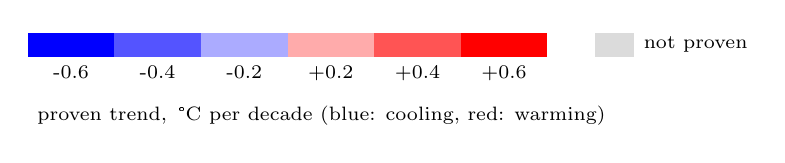
\begin{tikzpicture}
\fill[blue!100!white] (0.00,0) rectangle ++(1.1,0.3); \node[below, font=\scriptsize] at (0.55,0) {-0.6};
\fill[blue!67!white] (1.10,0) rectangle ++(1.1,0.3); \node[below, font=\scriptsize] at (1.65,0) {-0.4};
\fill[blue!33!white] (2.20,0) rectangle ++(1.1,0.3); \node[below, font=\scriptsize] at (2.75,0) {-0.2};
\fill[red!33!white] (3.30,0) rectangle ++(1.1,0.3); \node[below, font=\scriptsize] at (3.85,0) {+0.2};
\fill[red!67!white] (4.40,0) rectangle ++(1.1,0.3); \node[below, font=\scriptsize] at (4.95,0) {+0.4};
\fill[red!100!white] (5.50,0) rectangle ++(1.1,0.3); \node[below, font=\scriptsize] at (6.05,0) {+0.6};
\fill[black!14] (7.2,0) rectangle ++(0.5,0.3); \node[right, font=\scriptsize] at (7.7,0.15) {not proven};
\node[font=\scriptsize, anchor=west] at (0,-0.75) {proven trend, \degC{} per decade (blue: cooling, red: warming)};
\end{tikzpicture}
\caption{Air temperature trend 2001--2025 per 55\,km grid cell (NASA POWER), after false discovery control. Coloured cells: proven trend; grey: not proven.}\label{fig:maps}
\end{figure}

\begin{figure}[h]\centering
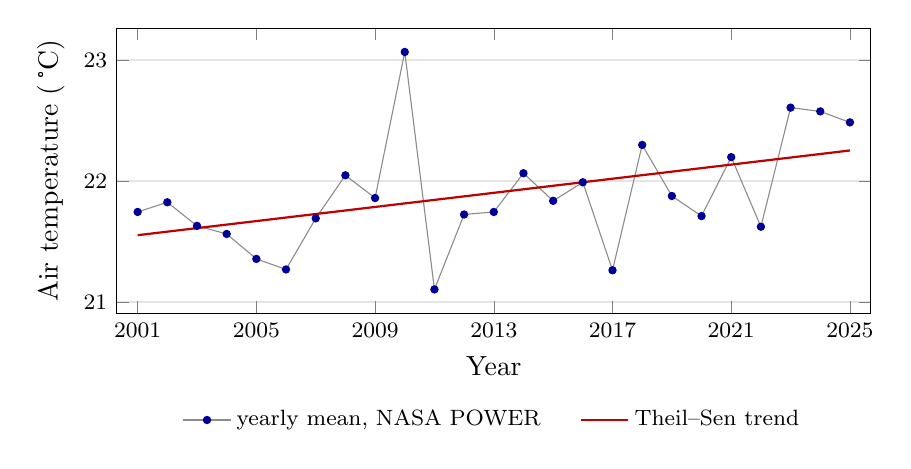
\begin{tikzpicture}
\begin{axis}[width=0.92\linewidth, height=5.2cm, xmin=2000.3, xmax=2025.7,
  xlabel={Year}, ylabel={Air temperature (\degC)}, xtick={2001,2005,...,2025},
  x tick label style={/pgf/number format/1000 sep={}}, ymajorgrids, grid style={black!10},
  legend style={font=\footnotesize, draw=none, at={(0.5,-0.3)}, anchor=north, legend columns=2, /tikz/every even column/.append style={column sep=12pt}}, tick label style={font=\footnotesize}]
\addplot[black!45, thin, mark=*, mark size=1.3pt, mark options={fill=blue!60!black, draw=blue!60!black}] coordinates {(2001,21.744) (2002,21.824) (2003,21.629) (2004,21.562) (2005,21.356) (2006,21.269) (2007,21.691) (2008,22.047) (2009,21.859) (2010,23.066) (2011,21.104) (2012,21.723) (2013,21.744) (2014,22.064) (2015,21.836) (2016,21.989) (2017,21.262) (2018,22.298) (2019,21.876) (2020,21.710) (2021,22.197) (2022,21.622) (2023,22.606) (2024,22.575) (2025,22.484)};
\addlegendentry{yearly mean, NASA POWER}
\addplot[red!75!black, thick] coordinates {(2001,21.552) (2025,22.252)};
\addlegendentry{Theil--Sen trend}
\end{axis}
\end{tikzpicture}
\caption{Cairo: yearly mean air temperature from NASA POWER and its Theil--Sen trend.}\label{fig:cairo}
\end{figure}

\subsection{A problem in the rain record}\label{sec:rain}
While checking rainfall we found that POWER's precipitation over Egypt's farmland jumps around 2015: the mean after 2015 is about 2.6 times the mean before (Pettitt test, $p<0.001$). GPCP, which uses satellites and gauges, rises only 1.24 times at the same places. The jump is therefore in the dataset rather than in the sky. A naive trend test would have reported a dramatic, ``highly significant'' increase in rain. Instead, every rain answer in the app carries a caution, and the crop projections remove this one-time step before measuring the trend.

\subsection{Crop suitability}
Table~\ref{tab:crop} summarises the crop model on regions held out of training. Trained without any Egyptian data, it still separates the crops Egypt grows from those it does not (FAOSTAT) with an AUC of 0.93. Where Egypt actually grows them, irrigated scores (0 to 100) are high for the main crops: wheat 94, tomato 90, maize 79 and rice 75. Under continued trends the average change in crop scores on Egypt's farmland by 2035 is small, about 1.3 points. The model does not represent water supply, so this should not be read as an absence of risk for Egyptian farming.

\begin{table}[h]\centering\small
\caption{Crop model performance on held-out regions, mean over 40 crops.}\label{tab:crop}
\begin{tabular}{@{}lc@{}}
\toprule
Measure & Value \\
\midrule
AUC, all / irrigated / rain-fed farmland & 0.90 / 0.85 / 0.88 \\
Worst single crop, AUC & 0.82 \\
True skill statistic / Brier score / calibration error & 0.64 / 0.13 / 0.04 \\
Trained without Egypt: Egypt's crop list (FAOSTAT), AUC & 0.93 \\
Rain only: crops rated suitable in unfarmed deserts & 0 \\
\bottomrule
\end{tabular}
\end{table}

\section{Discussion and limitations}
The main strength of the approach is that a ``proven'' label has a measured meaning: we know how often our test raises a false alarm, and every map is corrected for testing many places at once. The price is caution. Over a 25-year record with realistic persistence, moderate trends are often not proven, and in Egypt POWER is more conservative than the station record. We think it is better to say ``not proven'' and show the station evidence than to colour the whole country red.

There are several limitations. The grid cells are about 55\,km wide, so the tool is suited to regional screening rather than decisions about a single farm. Irrigated mode assumes water can be supplied and does not show whether it exists. The crop model learns where crops are grown today, which reflects markets, policy and water as well as climate, and olive and date palm are not separate crops in MapSPAM. Projections only continue present trends and are not climate forecasts. Finally, the free hosting sleeps after 15 minutes without visitors, so the first visit can take about a minute.

\section{Future work}
The next steps are finer satellite layers (MODIS and VIIRS at 1\,km) to see individual fields and towns; water availability from NASA GRACE groundwater and river records, so that irrigated answers can say where water exists; heat extremes, such as the number of very hot days, next to the averages; an Arabic interface; and more countries for the farming tabs.

\section{Conclusion}
CropShift Earth answers the challenge's questions (what is changing, where, how much and whether it is significant) for any place on Earth, and it shows opposite trends inside a single country. Its statistics were chosen on evidence and checked against independent NASA records, which also revealed a problem in the rain data that would otherwise have produced a false result. By linking established trends to crop suitability for 20 countries, it turns a climate question into one that farmers and planners in our region can act on.

\section*{Data and resources}
\small
\begin{tabularx}{\linewidth}{@{}p{0.34\linewidth}X@{}}
\toprule
\multicolumn{2}{@{}l}{\textbf{NASA data}} \\
\midrule
NASA POWER, monthly, 2001--2025 & All maps, charts and crop scores. \url{https://power.larc.nasa.gov} \\
NASA GMAO MERRA-2 & Reanalysis behind POWER. \url{https://gmao.gsfc.nasa.gov/reanalysis/MERRA-2/} \\
NASA GISTEMP v4 & Validation; station trend shown in the app. \url{https://data.giss.nasa.gov/gistemp/} \\
GPCP v2.3 (NASA GSFC led) & Independent rain check. \url{https://psl.noaa.gov/data/gridded/data.gpcp.html} \\
NASA GIBS & Globe imagery (Blue Marble, VIIRS). \url{https://earthdata.nasa.gov/gibs} \\
\midrule
\multicolumn{2}{@{}l}{\textbf{Other data and resources}} \\
\midrule
IFPRI MapSPAM 2020 v2r2 (CC BY 4.0) & Crop model labels. \url{https://doi.org/10.7910/DVN/SWPENT}. \emph{This data was provided by the International Food Policy Research Institute (IFPRI). IFPRI bears no responsibility for the analyses or interpretations of the data presented here.} \\
FAOSTAT; FAO ECOCROP & Crop list check; first crop calculator. \url{https://www.fao.org/faostat/} \\
Natural Earth & Borders and cities. \url{https://www.naturalearthdata.com} \\
Sentinel-2 cloudless by EOX & Close-up imagery (contains modified Copernicus Sentinel data 2020). \url{https://s2maps.eu} \\
Software & Python, FastAPI, NumPy, pandas, SciPy, statsmodels, pymannkendall, XGBoost, scikit-learn, MapLibre GL JS, Plotly.js; GitHub, Render, Hugging Face, Kaggle. Full list: \texttt{docs/REFERENCES.md} in the repository. \\
\bottomrule
\end{tabularx}
\normalsize

\section*{Use of AI tools}
We used AI assistants during the hackathon and state where. Claude (Anthropic) helped write and debug code across the analysis, server and interface, drafted analysis scripts and checks, summarised background research and helped draft documentation, including this report. Manus, an AI agent, wrote the first training notebook of the crop model on Kaggle; the model used in the app was retrained from it in our repository. All AI-assisted code and text were reviewed by the team and the code is covered by automated tests. The crop model itself is a conventional machine learning model trained by us on public data, and no language model generates any number shown in the app: every sentence is assembled from computed values. The figures in this report are drawn by our own script from the live application's results. No NASA logos or branding are used.

\begin{thebibliography}{99}\small
\bibitem{adler2018} R.\,F. Adler et al. The Global Precipitation Climatology Project (GPCP) monthly analysis (new version 2.3) and a review of 2017 global precipitation. \emph{Atmosphere}, 9(4):138, 2018.
\bibitem{bh1995} Y. Benjamini and Y. Hochberg. Controlling the false discovery rate: a practical and powerful approach to multiple testing. \emph{J. R. Stat. Soc. B}, 57:289--300, 1995.
\bibitem{chen2016} T. Chen and C. Guestrin. XGBoost: a scalable tree boosting system. In \emph{Proc. KDD}, 785--794, 2016.
\bibitem{faostat} FAO. FAOSTAT: crops and livestock products. \url{https://www.fao.org/faostat/}, accessed 2026.
\bibitem{gelaro2017} R. Gelaro et al. The Modern-Era Retrospective Analysis for Research and Applications, Version 2 (MERRA-2). \emph{J. Climate}, 30:5419--5454, 2017.
\bibitem{hamed1998} K.\,H. Hamed and A.\,R. Rao. A modified Mann--Kendall trend test for autocorrelated data. \emph{J. Hydrology}, 204:182--196, 1998.
\bibitem{kendall1975} M.\,G. Kendall. \emph{Rank Correlation Methods}. Griffin, London, 1975.
\bibitem{lenssen2019} N. Lenssen et al. Improvements in the GISTEMP uncertainty model. \emph{J. Geophys. Res. Atmos.}, 124:6307--6326, 2019.
\bibitem{mann1945} H.\,B. Mann. Nonparametric tests against trend. \emph{Econometrica}, 13:245--259, 1945.
\bibitem{medecc2020} MedECC. \emph{Climate and Environmental Change in the Mediterranean Basin: Current Situation and Risks for the Future}. First Mediterranean Assessment Report, 2020.
\bibitem{owid} Our World in Data, based on ILO modelled estimates. Share of employment in agriculture. \url{https://ourworldindata.org/grapher/share-of-the-labor-force-employed-in-agriculture}, accessed November 2026.
\bibitem{pettitt1979} A.\,N. Pettitt. A non-parametric approach to the change-point problem. \emph{Applied Statistics}, 28:126--135, 1979.
\bibitem{power} NASA Langley Research Center. Prediction Of Worldwide Energy Resources (POWER). \url{https://power.larc.nasa.gov}, accessed 2026.
\bibitem{sen1968} P.\,K. Sen. Estimates of the regression coefficient based on Kendall's tau. \emph{J. Am. Stat. Assoc.}, 63:1379--1389, 1968.
\bibitem{spam2020} International Food Policy Research Institute. Global spatially-disaggregated crop production statistics data for 2020, version 2.0 release 2 (SPAM 2020 v2r2). Harvard Dataverse, 2026. \url{https://doi.org/10.7910/DVN/SWPENT}
\bibitem{wilks2016} D.\,S. Wilks. ``The stippling shows statistically significant grid points'': how research results are routinely overstated and overinterpreted, and what to do about it. \emph{Bull. Amer. Meteor. Soc.}, 97:2263--2273, 2016.
\bibitem{worldbank2018} World Bank. \emph{Beyond Scarcity: Water Security in the Middle East and North Africa}. Washington, DC, 2018.
\bibitem{yue2004} S. Yue and C.\,Y. Wang. The Mann--Kendall test modified by effective sample size to detect trend in serially correlated hydrological series. \emph{Water Resources Management}, 18:201--218, 2004.
\end{thebibliography}

\end{document}
